\documentclass[11pt]{article}

    \usepackage[breakable]{tcolorbox}
    \usepackage{parskip} % Stop auto-indenting (to mimic markdown behaviour)
    
    \usepackage{iftex}
    \ifPDFTeX
    	\usepackage[T1]{fontenc}
    	\usepackage{mathpazo}
    \else
    	\usepackage{fontspec}
    \fi

    % Basic figure setup, for now with no caption control since it's done
    % automatically by Pandoc (which extracts ![](path) syntax from Markdown).
    \usepackage{graphicx}
    % Maintain compatibility with old templates. Remove in nbconvert 6.0
    \let\Oldincludegraphics\includegraphics
    % Ensure that by default, figures have no caption (until we provide a
    % proper Figure object with a Caption API and a way to capture that
    % in the conversion process - todo).
    \usepackage{caption}
    \DeclareCaptionFormat{nocaption}{}
    \captionsetup{format=nocaption,aboveskip=0pt,belowskip=0pt}

    \usepackage[Export]{adjustbox} % Used to constrain images to a maximum size
    \adjustboxset{max size={0.9\linewidth}{0.9\paperheight}}
    \usepackage{float}
    \floatplacement{figure}{H} % forces figures to be placed at the correct location
    \usepackage{xcolor} % Allow colors to be defined
    \usepackage{enumerate} % Needed for markdown enumerations to work
    \usepackage{geometry} % Used to adjust the document margins
    \usepackage{amsmath} % Equations
    \usepackage{amssymb} % Equations
    \usepackage{textcomp} % defines textquotesingle
    % Hack from http://tex.stackexchange.com/a/47451/13684:
    \AtBeginDocument{%
        \def\PYZsq{\textquotesingle}% Upright quotes in Pygmentized code
    }
    \usepackage{upquote} % Upright quotes for verbatim code
    \usepackage{eurosym} % defines \euro
    \usepackage[mathletters]{ucs} % Extended unicode (utf-8) support
    \usepackage{fancyvrb} % verbatim replacement that allows latex

    % The hyperref package gives us a pdf with properly built
    % internal navigation ('pdf bookmarks' for the table of contents,
    % internal cross-reference links, web links for URLs, etc.)
    \usepackage{hyperref}
    % The default LaTeX title has an obnoxious amount of whitespace. By default,
    % titling removes some of it. It also provides customization options.
    \usepackage{titling}
    \usepackage{longtable} % longtable support required by pandoc >1.10
    \usepackage{booktabs}  % table support for pandoc > 1.12.2
    \usepackage[inline]{enumitem} % IRkernel/repr support (it uses the enumerate* environment)
    \usepackage[normalem]{ulem} % ulem is needed to support strikethroughs (\sout)
                                % normalem makes italics be italics, not underlines
    \usepackage{mathrsfs}
    

    
    % Colors for the hyperref package
    \definecolor{urlcolor}{rgb}{0,.145,.698}
    \definecolor{linkcolor}{rgb}{.71,0.21,0.01}
    \definecolor{citecolor}{rgb}{.12,.54,.11}

    % ANSI colors
    \definecolor{ansi-black}{HTML}{3E424D}
    \definecolor{ansi-black-intense}{HTML}{282C36}
    \definecolor{ansi-red}{HTML}{E75C58}
    \definecolor{ansi-red-intense}{HTML}{B22B31}
    \definecolor{ansi-green}{HTML}{00A250}
    \definecolor{ansi-green-intense}{HTML}{007427}
    \definecolor{ansi-yellow}{HTML}{DDB62B}
    \definecolor{ansi-yellow-intense}{HTML}{B27D12}
    \definecolor{ansi-blue}{HTML}{208FFB}
    \definecolor{ansi-blue-intense}{HTML}{0065CA}
    \definecolor{ansi-magenta}{HTML}{D160C4}
    \definecolor{ansi-magenta-intense}{HTML}{A03196}
    \definecolor{ansi-cyan}{HTML}{60C6C8}
    \definecolor{ansi-cyan-intense}{HTML}{258F8F}
    \definecolor{ansi-white}{HTML}{C5C1B4}
    \definecolor{ansi-white-intense}{HTML}{A1A6B2}
    \definecolor{ansi-default-inverse-fg}{HTML}{FFFFFF}
    \definecolor{ansi-default-inverse-bg}{HTML}{000000}

    % commands and environments needed by pandoc snippets
    % extracted from the output of `pandoc -s`
    \providecommand{\tightlist}{%
      \setlength{\itemsep}{0pt}\setlength{\parskip}{0pt}}
    \DefineVerbatimEnvironment{Highlighting}{Verbatim}{commandchars=\\\{\}}
    % Add ',fontsize=\small' for more characters per line
    \newenvironment{Shaded}{}{}
    \newcommand{\KeywordTok}[1]{\textcolor[rgb]{0.00,0.44,0.13}{\textbf{{#1}}}}
    \newcommand{\DataTypeTok}[1]{\textcolor[rgb]{0.56,0.13,0.00}{{#1}}}
    \newcommand{\DecValTok}[1]{\textcolor[rgb]{0.25,0.63,0.44}{{#1}}}
    \newcommand{\BaseNTok}[1]{\textcolor[rgb]{0.25,0.63,0.44}{{#1}}}
    \newcommand{\FloatTok}[1]{\textcolor[rgb]{0.25,0.63,0.44}{{#1}}}
    \newcommand{\CharTok}[1]{\textcolor[rgb]{0.25,0.44,0.63}{{#1}}}
    \newcommand{\StringTok}[1]{\textcolor[rgb]{0.25,0.44,0.63}{{#1}}}
    \newcommand{\CommentTok}[1]{\textcolor[rgb]{0.38,0.63,0.69}{\textit{{#1}}}}
    \newcommand{\OtherTok}[1]{\textcolor[rgb]{0.00,0.44,0.13}{{#1}}}
    \newcommand{\AlertTok}[1]{\textcolor[rgb]{1.00,0.00,0.00}{\textbf{{#1}}}}
    \newcommand{\FunctionTok}[1]{\textcolor[rgb]{0.02,0.16,0.49}{{#1}}}
    \newcommand{\RegionMarkerTok}[1]{{#1}}
    \newcommand{\ErrorTok}[1]{\textcolor[rgb]{1.00,0.00,0.00}{\textbf{{#1}}}}
    \newcommand{\NormalTok}[1]{{#1}}
    
    % Additional commands for more recent versions of Pandoc
    \newcommand{\ConstantTok}[1]{\textcolor[rgb]{0.53,0.00,0.00}{{#1}}}
    \newcommand{\SpecialCharTok}[1]{\textcolor[rgb]{0.25,0.44,0.63}{{#1}}}
    \newcommand{\VerbatimStringTok}[1]{\textcolor[rgb]{0.25,0.44,0.63}{{#1}}}
    \newcommand{\SpecialStringTok}[1]{\textcolor[rgb]{0.73,0.40,0.53}{{#1}}}
    \newcommand{\ImportTok}[1]{{#1}}
    \newcommand{\DocumentationTok}[1]{\textcolor[rgb]{0.73,0.13,0.13}{\textit{{#1}}}}
    \newcommand{\AnnotationTok}[1]{\textcolor[rgb]{0.38,0.63,0.69}{\textbf{\textit{{#1}}}}}
    \newcommand{\CommentVarTok}[1]{\textcolor[rgb]{0.38,0.63,0.69}{\textbf{\textit{{#1}}}}}
    \newcommand{\VariableTok}[1]{\textcolor[rgb]{0.10,0.09,0.49}{{#1}}}
    \newcommand{\ControlFlowTok}[1]{\textcolor[rgb]{0.00,0.44,0.13}{\textbf{{#1}}}}
    \newcommand{\OperatorTok}[1]{\textcolor[rgb]{0.40,0.40,0.40}{{#1}}}
    \newcommand{\BuiltInTok}[1]{{#1}}
    \newcommand{\ExtensionTok}[1]{{#1}}
    \newcommand{\PreprocessorTok}[1]{\textcolor[rgb]{0.74,0.48,0.00}{{#1}}}
    \newcommand{\AttributeTok}[1]{\textcolor[rgb]{0.49,0.56,0.16}{{#1}}}
    \newcommand{\InformationTok}[1]{\textcolor[rgb]{0.38,0.63,0.69}{\textbf{\textit{{#1}}}}}
    \newcommand{\WarningTok}[1]{\textcolor[rgb]{0.38,0.63,0.69}{\textbf{\textit{{#1}}}}}
    
    
    % Define a nice break command that doesn't care if a line doesn't already
    % exist.
    \def\br{\hspace*{\fill} \\* }
    % Math Jax compatibility definitions
    \def\gt{>}
    \def\lt{<}
    \let\Oldtex\TeX
    \let\Oldlatex\LaTeX
    \renewcommand{\TeX}{\textrm{\Oldtex}}
    \renewcommand{\LaTeX}{\textrm{\Oldlatex}}
    % Document parameters
    % Document title
    \title{tuto\_install\_debian}
    
    
    
    
    
% Pygments definitions
\makeatletter
\def\PY@reset{\let\PY@it=\relax \let\PY@bf=\relax%
    \let\PY@ul=\relax \let\PY@tc=\relax%
    \let\PY@bc=\relax \let\PY@ff=\relax}
\def\PY@tok#1{\csname PY@tok@#1\endcsname}
\def\PY@toks#1+{\ifx\relax#1\empty\else%
    \PY@tok{#1}\expandafter\PY@toks\fi}
\def\PY@do#1{\PY@bc{\PY@tc{\PY@ul{%
    \PY@it{\PY@bf{\PY@ff{#1}}}}}}}
\def\PY#1#2{\PY@reset\PY@toks#1+\relax+\PY@do{#2}}

\expandafter\def\csname PY@tok@w\endcsname{\def\PY@tc##1{\textcolor[rgb]{0.73,0.73,0.73}{##1}}}
\expandafter\def\csname PY@tok@c\endcsname{\let\PY@it=\textit\def\PY@tc##1{\textcolor[rgb]{0.25,0.50,0.50}{##1}}}
\expandafter\def\csname PY@tok@cp\endcsname{\def\PY@tc##1{\textcolor[rgb]{0.74,0.48,0.00}{##1}}}
\expandafter\def\csname PY@tok@k\endcsname{\let\PY@bf=\textbf\def\PY@tc##1{\textcolor[rgb]{0.00,0.50,0.00}{##1}}}
\expandafter\def\csname PY@tok@kp\endcsname{\def\PY@tc##1{\textcolor[rgb]{0.00,0.50,0.00}{##1}}}
\expandafter\def\csname PY@tok@kt\endcsname{\def\PY@tc##1{\textcolor[rgb]{0.69,0.00,0.25}{##1}}}
\expandafter\def\csname PY@tok@o\endcsname{\def\PY@tc##1{\textcolor[rgb]{0.40,0.40,0.40}{##1}}}
\expandafter\def\csname PY@tok@ow\endcsname{\let\PY@bf=\textbf\def\PY@tc##1{\textcolor[rgb]{0.67,0.13,1.00}{##1}}}
\expandafter\def\csname PY@tok@nb\endcsname{\def\PY@tc##1{\textcolor[rgb]{0.00,0.50,0.00}{##1}}}
\expandafter\def\csname PY@tok@nf\endcsname{\def\PY@tc##1{\textcolor[rgb]{0.00,0.00,1.00}{##1}}}
\expandafter\def\csname PY@tok@nc\endcsname{\let\PY@bf=\textbf\def\PY@tc##1{\textcolor[rgb]{0.00,0.00,1.00}{##1}}}
\expandafter\def\csname PY@tok@nn\endcsname{\let\PY@bf=\textbf\def\PY@tc##1{\textcolor[rgb]{0.00,0.00,1.00}{##1}}}
\expandafter\def\csname PY@tok@ne\endcsname{\let\PY@bf=\textbf\def\PY@tc##1{\textcolor[rgb]{0.82,0.25,0.23}{##1}}}
\expandafter\def\csname PY@tok@nv\endcsname{\def\PY@tc##1{\textcolor[rgb]{0.10,0.09,0.49}{##1}}}
\expandafter\def\csname PY@tok@no\endcsname{\def\PY@tc##1{\textcolor[rgb]{0.53,0.00,0.00}{##1}}}
\expandafter\def\csname PY@tok@nl\endcsname{\def\PY@tc##1{\textcolor[rgb]{0.63,0.63,0.00}{##1}}}
\expandafter\def\csname PY@tok@ni\endcsname{\let\PY@bf=\textbf\def\PY@tc##1{\textcolor[rgb]{0.60,0.60,0.60}{##1}}}
\expandafter\def\csname PY@tok@na\endcsname{\def\PY@tc##1{\textcolor[rgb]{0.49,0.56,0.16}{##1}}}
\expandafter\def\csname PY@tok@nt\endcsname{\let\PY@bf=\textbf\def\PY@tc##1{\textcolor[rgb]{0.00,0.50,0.00}{##1}}}
\expandafter\def\csname PY@tok@nd\endcsname{\def\PY@tc##1{\textcolor[rgb]{0.67,0.13,1.00}{##1}}}
\expandafter\def\csname PY@tok@s\endcsname{\def\PY@tc##1{\textcolor[rgb]{0.73,0.13,0.13}{##1}}}
\expandafter\def\csname PY@tok@sd\endcsname{\let\PY@it=\textit\def\PY@tc##1{\textcolor[rgb]{0.73,0.13,0.13}{##1}}}
\expandafter\def\csname PY@tok@si\endcsname{\let\PY@bf=\textbf\def\PY@tc##1{\textcolor[rgb]{0.73,0.40,0.53}{##1}}}
\expandafter\def\csname PY@tok@se\endcsname{\let\PY@bf=\textbf\def\PY@tc##1{\textcolor[rgb]{0.73,0.40,0.13}{##1}}}
\expandafter\def\csname PY@tok@sr\endcsname{\def\PY@tc##1{\textcolor[rgb]{0.73,0.40,0.53}{##1}}}
\expandafter\def\csname PY@tok@ss\endcsname{\def\PY@tc##1{\textcolor[rgb]{0.10,0.09,0.49}{##1}}}
\expandafter\def\csname PY@tok@sx\endcsname{\def\PY@tc##1{\textcolor[rgb]{0.00,0.50,0.00}{##1}}}
\expandafter\def\csname PY@tok@m\endcsname{\def\PY@tc##1{\textcolor[rgb]{0.40,0.40,0.40}{##1}}}
\expandafter\def\csname PY@tok@gh\endcsname{\let\PY@bf=\textbf\def\PY@tc##1{\textcolor[rgb]{0.00,0.00,0.50}{##1}}}
\expandafter\def\csname PY@tok@gu\endcsname{\let\PY@bf=\textbf\def\PY@tc##1{\textcolor[rgb]{0.50,0.00,0.50}{##1}}}
\expandafter\def\csname PY@tok@gd\endcsname{\def\PY@tc##1{\textcolor[rgb]{0.63,0.00,0.00}{##1}}}
\expandafter\def\csname PY@tok@gi\endcsname{\def\PY@tc##1{\textcolor[rgb]{0.00,0.63,0.00}{##1}}}
\expandafter\def\csname PY@tok@gr\endcsname{\def\PY@tc##1{\textcolor[rgb]{1.00,0.00,0.00}{##1}}}
\expandafter\def\csname PY@tok@ge\endcsname{\let\PY@it=\textit}
\expandafter\def\csname PY@tok@gs\endcsname{\let\PY@bf=\textbf}
\expandafter\def\csname PY@tok@gp\endcsname{\let\PY@bf=\textbf\def\PY@tc##1{\textcolor[rgb]{0.00,0.00,0.50}{##1}}}
\expandafter\def\csname PY@tok@go\endcsname{\def\PY@tc##1{\textcolor[rgb]{0.53,0.53,0.53}{##1}}}
\expandafter\def\csname PY@tok@gt\endcsname{\def\PY@tc##1{\textcolor[rgb]{0.00,0.27,0.87}{##1}}}
\expandafter\def\csname PY@tok@err\endcsname{\def\PY@bc##1{\setlength{\fboxsep}{0pt}\fcolorbox[rgb]{1.00,0.00,0.00}{1,1,1}{\strut ##1}}}
\expandafter\def\csname PY@tok@kc\endcsname{\let\PY@bf=\textbf\def\PY@tc##1{\textcolor[rgb]{0.00,0.50,0.00}{##1}}}
\expandafter\def\csname PY@tok@kd\endcsname{\let\PY@bf=\textbf\def\PY@tc##1{\textcolor[rgb]{0.00,0.50,0.00}{##1}}}
\expandafter\def\csname PY@tok@kn\endcsname{\let\PY@bf=\textbf\def\PY@tc##1{\textcolor[rgb]{0.00,0.50,0.00}{##1}}}
\expandafter\def\csname PY@tok@kr\endcsname{\let\PY@bf=\textbf\def\PY@tc##1{\textcolor[rgb]{0.00,0.50,0.00}{##1}}}
\expandafter\def\csname PY@tok@bp\endcsname{\def\PY@tc##1{\textcolor[rgb]{0.00,0.50,0.00}{##1}}}
\expandafter\def\csname PY@tok@fm\endcsname{\def\PY@tc##1{\textcolor[rgb]{0.00,0.00,1.00}{##1}}}
\expandafter\def\csname PY@tok@vc\endcsname{\def\PY@tc##1{\textcolor[rgb]{0.10,0.09,0.49}{##1}}}
\expandafter\def\csname PY@tok@vg\endcsname{\def\PY@tc##1{\textcolor[rgb]{0.10,0.09,0.49}{##1}}}
\expandafter\def\csname PY@tok@vi\endcsname{\def\PY@tc##1{\textcolor[rgb]{0.10,0.09,0.49}{##1}}}
\expandafter\def\csname PY@tok@vm\endcsname{\def\PY@tc##1{\textcolor[rgb]{0.10,0.09,0.49}{##1}}}
\expandafter\def\csname PY@tok@sa\endcsname{\def\PY@tc##1{\textcolor[rgb]{0.73,0.13,0.13}{##1}}}
\expandafter\def\csname PY@tok@sb\endcsname{\def\PY@tc##1{\textcolor[rgb]{0.73,0.13,0.13}{##1}}}
\expandafter\def\csname PY@tok@sc\endcsname{\def\PY@tc##1{\textcolor[rgb]{0.73,0.13,0.13}{##1}}}
\expandafter\def\csname PY@tok@dl\endcsname{\def\PY@tc##1{\textcolor[rgb]{0.73,0.13,0.13}{##1}}}
\expandafter\def\csname PY@tok@s2\endcsname{\def\PY@tc##1{\textcolor[rgb]{0.73,0.13,0.13}{##1}}}
\expandafter\def\csname PY@tok@sh\endcsname{\def\PY@tc##1{\textcolor[rgb]{0.73,0.13,0.13}{##1}}}
\expandafter\def\csname PY@tok@s1\endcsname{\def\PY@tc##1{\textcolor[rgb]{0.73,0.13,0.13}{##1}}}
\expandafter\def\csname PY@tok@mb\endcsname{\def\PY@tc##1{\textcolor[rgb]{0.40,0.40,0.40}{##1}}}
\expandafter\def\csname PY@tok@mf\endcsname{\def\PY@tc##1{\textcolor[rgb]{0.40,0.40,0.40}{##1}}}
\expandafter\def\csname PY@tok@mh\endcsname{\def\PY@tc##1{\textcolor[rgb]{0.40,0.40,0.40}{##1}}}
\expandafter\def\csname PY@tok@mi\endcsname{\def\PY@tc##1{\textcolor[rgb]{0.40,0.40,0.40}{##1}}}
\expandafter\def\csname PY@tok@il\endcsname{\def\PY@tc##1{\textcolor[rgb]{0.40,0.40,0.40}{##1}}}
\expandafter\def\csname PY@tok@mo\endcsname{\def\PY@tc##1{\textcolor[rgb]{0.40,0.40,0.40}{##1}}}
\expandafter\def\csname PY@tok@ch\endcsname{\let\PY@it=\textit\def\PY@tc##1{\textcolor[rgb]{0.25,0.50,0.50}{##1}}}
\expandafter\def\csname PY@tok@cm\endcsname{\let\PY@it=\textit\def\PY@tc##1{\textcolor[rgb]{0.25,0.50,0.50}{##1}}}
\expandafter\def\csname PY@tok@cpf\endcsname{\let\PY@it=\textit\def\PY@tc##1{\textcolor[rgb]{0.25,0.50,0.50}{##1}}}
\expandafter\def\csname PY@tok@c1\endcsname{\let\PY@it=\textit\def\PY@tc##1{\textcolor[rgb]{0.25,0.50,0.50}{##1}}}
\expandafter\def\csname PY@tok@cs\endcsname{\let\PY@it=\textit\def\PY@tc##1{\textcolor[rgb]{0.25,0.50,0.50}{##1}}}

\def\PYZbs{\char`\\}
\def\PYZus{\char`\_}
\def\PYZob{\char`\{}
\def\PYZcb{\char`\}}
\def\PYZca{\char`\^}
\def\PYZam{\char`\&}
\def\PYZlt{\char`\<}
\def\PYZgt{\char`\>}
\def\PYZsh{\char`\#}
\def\PYZpc{\char`\%}
\def\PYZdl{\char`\$}
\def\PYZhy{\char`\-}
\def\PYZsq{\char`\'}
\def\PYZdq{\char`\"}
\def\PYZti{\char`\~}
% for compatibility with earlier versions
\def\PYZat{@}
\def\PYZlb{[}
\def\PYZrb{]}
\makeatother


    % For linebreaks inside Verbatim environment from package fancyvrb. 
    \makeatletter
        \newbox\Wrappedcontinuationbox 
        \newbox\Wrappedvisiblespacebox 
        \newcommand*\Wrappedvisiblespace {\textcolor{red}{\textvisiblespace}} 
        \newcommand*\Wrappedcontinuationsymbol {\textcolor{red}{\llap{\tiny$\m@th\hookrightarrow$}}} 
        \newcommand*\Wrappedcontinuationindent {3ex } 
        \newcommand*\Wrappedafterbreak {\kern\Wrappedcontinuationindent\copy\Wrappedcontinuationbox} 
        % Take advantage of the already applied Pygments mark-up to insert 
        % potential linebreaks for TeX processing. 
        %        {, <, #, %, $, ' and ": go to next line. 
        %        _, }, ^, &, >, - and ~: stay at end of broken line. 
        % Use of \textquotesingle for straight quote. 
        \newcommand*\Wrappedbreaksatspecials {% 
            \def\PYGZus{\discretionary{\char`\_}{\Wrappedafterbreak}{\char`\_}}% 
            \def\PYGZob{\discretionary{}{\Wrappedafterbreak\char`\{}{\char`\{}}% 
            \def\PYGZcb{\discretionary{\char`\}}{\Wrappedafterbreak}{\char`\}}}% 
            \def\PYGZca{\discretionary{\char`\^}{\Wrappedafterbreak}{\char`\^}}% 
            \def\PYGZam{\discretionary{\char`\&}{\Wrappedafterbreak}{\char`\&}}% 
            \def\PYGZlt{\discretionary{}{\Wrappedafterbreak\char`\<}{\char`\<}}% 
            \def\PYGZgt{\discretionary{\char`\>}{\Wrappedafterbreak}{\char`\>}}% 
            \def\PYGZsh{\discretionary{}{\Wrappedafterbreak\char`\#}{\char`\#}}% 
            \def\PYGZpc{\discretionary{}{\Wrappedafterbreak\char`\%}{\char`\%}}% 
            \def\PYGZdl{\discretionary{}{\Wrappedafterbreak\char`\$}{\char`\$}}% 
            \def\PYGZhy{\discretionary{\char`\-}{\Wrappedafterbreak}{\char`\-}}% 
            \def\PYGZsq{\discretionary{}{\Wrappedafterbreak\textquotesingle}{\textquotesingle}}% 
            \def\PYGZdq{\discretionary{}{\Wrappedafterbreak\char`\"}{\char`\"}}% 
            \def\PYGZti{\discretionary{\char`\~}{\Wrappedafterbreak}{\char`\~}}% 
        } 
        % Some characters . , ; ? ! / are not pygmentized. 
        % This macro makes them "active" and they will insert potential linebreaks 
        \newcommand*\Wrappedbreaksatpunct {% 
            \lccode`\~`\.\lowercase{\def~}{\discretionary{\hbox{\char`\.}}{\Wrappedafterbreak}{\hbox{\char`\.}}}% 
            \lccode`\~`\,\lowercase{\def~}{\discretionary{\hbox{\char`\,}}{\Wrappedafterbreak}{\hbox{\char`\,}}}% 
            \lccode`\~`\;\lowercase{\def~}{\discretionary{\hbox{\char`\;}}{\Wrappedafterbreak}{\hbox{\char`\;}}}% 
            \lccode`\~`\:\lowercase{\def~}{\discretionary{\hbox{\char`\:}}{\Wrappedafterbreak}{\hbox{\char`\:}}}% 
            \lccode`\~`\?\lowercase{\def~}{\discretionary{\hbox{\char`\?}}{\Wrappedafterbreak}{\hbox{\char`\?}}}% 
            \lccode`\~`\!\lowercase{\def~}{\discretionary{\hbox{\char`\!}}{\Wrappedafterbreak}{\hbox{\char`\!}}}% 
            \lccode`\~`\/\lowercase{\def~}{\discretionary{\hbox{\char`\/}}{\Wrappedafterbreak}{\hbox{\char`\/}}}% 
            \catcode`\.\active
            \catcode`\,\active 
            \catcode`\;\active
            \catcode`\:\active
            \catcode`\?\active
            \catcode`\!\active
            \catcode`\/\active 
            \lccode`\~`\~ 	
        }
    \makeatother

    \let\OriginalVerbatim=\Verbatim
    \makeatletter
    \renewcommand{\Verbatim}[1][1]{%
        %\parskip\z@skip
        \sbox\Wrappedcontinuationbox {\Wrappedcontinuationsymbol}%
        \sbox\Wrappedvisiblespacebox {\FV@SetupFont\Wrappedvisiblespace}%
        \def\FancyVerbFormatLine ##1{\hsize\linewidth
            \vtop{\raggedright\hyphenpenalty\z@\exhyphenpenalty\z@
                \doublehyphendemerits\z@\finalhyphendemerits\z@
                \strut ##1\strut}%
        }%
        % If the linebreak is at a space, the latter will be displayed as visible
        % space at end of first line, and a continuation symbol starts next line.
        % Stretch/shrink are however usually zero for typewriter font.
        \def\FV@Space {%
            \nobreak\hskip\z@ plus\fontdimen3\font minus\fontdimen4\font
            \discretionary{\copy\Wrappedvisiblespacebox}{\Wrappedafterbreak}
            {\kern\fontdimen2\font}%
        }%
        
        % Allow breaks at special characters using \PYG... macros.
        \Wrappedbreaksatspecials
        % Breaks at punctuation characters . , ; ? ! and / need catcode=\active 	
        \OriginalVerbatim[#1,codes*=\Wrappedbreaksatpunct]%
    }
    \makeatother

    % Exact colors from NB
    \definecolor{incolor}{HTML}{303F9F}
    \definecolor{outcolor}{HTML}{D84315}
    \definecolor{cellborder}{HTML}{CFCFCF}
    \definecolor{cellbackground}{HTML}{F7F7F7}
    
    % prompt
    \makeatletter
    \newcommand{\boxspacing}{\kern\kvtcb@left@rule\kern\kvtcb@boxsep}
    \makeatother
    \newcommand{\prompt}[4]{
        \ttfamily\llap{{\color{#2}[#3]:\hspace{3pt}#4}}\vspace{-\baselineskip}
    }
    

    
    % Prevent overflowing lines due to hard-to-break entities
    \sloppy 
    % Setup hyperref package
    \hypersetup{
      breaklinks=true,  % so long urls are correctly broken across lines
      colorlinks=true,
      urlcolor=urlcolor,
      linkcolor=linkcolor,
      citecolor=citecolor,
      }
    % Slightly bigger margins than the latex defaults
    
    \geometry{verbose,tmargin=1in,bmargin=1in,lmargin=1in,rmargin=1in}
    
    

\begin{document}
    
    \maketitle
    
    

    
    \hypertarget{installer-la-salle-202}{%
\section{Installer la salle 202}\label{installer-la-salle-202}}

    \hypertarget{questions-possibles}{%
\paragraph{Questions possibles}\label{questions-possibles}}

\begin{itemize}
\tightlist
\item
  Au démarrage d'un ordinateur, quel est le premier programme exécuté ?
\item
  Sur quoi est installé le système d'exploitation ?
\item
  Que signifie \emph{partitionner} un disque ?
\end{itemize}

    \hypertarget{installer-les-postes}{%
\subsection{Installer les postes}\label{installer-les-postes}}

    \begin{enumerate}
\def\labelenumi{\arabic{enumi}.}
\tightlist
\item
  Disjoncter
\item
  Pour chaque ligne de 3 tables, faire passer et ressortir

  \begin{itemize}
  \tightlist
  \item
    câble d'alimentation électrique
  \item
    câble réseau
  \end{itemize}
\item
  Placer :

  \begin{itemize}
  \tightlist
  \item
    écran
  \item
    clavier
  \item
    souris
  \end{itemize}
\item
  Positionner les unités centrales
\item
  Brancher et ranger les câbles
\end{enumerate}

    \hypertarget{installer-le-systuxe8me-dexploitation}{%
\subsection{Installer le système
d'exploitation}\label{installer-le-systuxe8me-dexploitation}}

    \hypertarget{configurer-le-bios}{%
\subsubsection{Configurer le BIOS}\label{configurer-le-bios}}

\begin{itemize}
\tightlist
\item
  brancher la clé USB
\item
  accéder au bios de la machine :

  \begin{itemize}
  \tightlist
  \item
    démarrer en appuyant sur \texttt{F12} (ou \texttt{F10} ou
    \texttt{Suppr.})
  \end{itemize}
\item
  changer l'ordre de lecture du système d'initialisation

  \begin{itemize}
  \tightlist
  \item
    mettre USB \textbf{en premier}
  \end{itemize}
\end{itemize}

    \hypertarget{partie-1---langue-et-utilisateurs}{%
\subsubsection{Partie 1 - Langue et
utilisateurs}\label{partie-1---langue-et-utilisateurs}}

    \begin{longtable}[]{@{}lll@{}}
\toprule
\endhead
\begin{minipage}[t]{0.27\columnwidth}\raggedright
1. Choisir l'installation graphique\\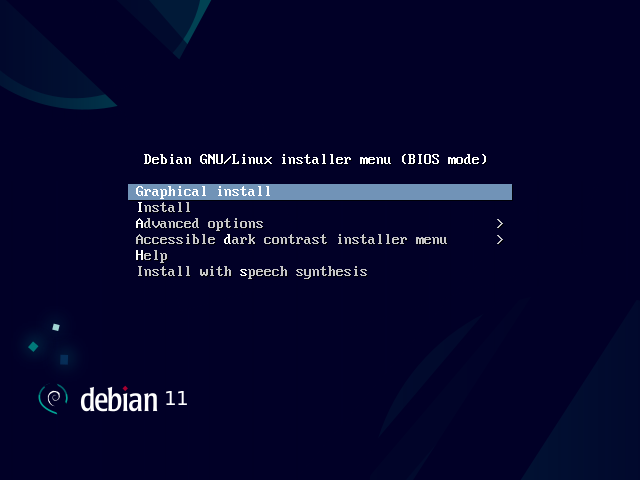
\includegraphics{res/01.png}\strut
\end{minipage} & \begin{minipage}[t]{0.37\columnwidth}\raggedright
2. Installation en français\\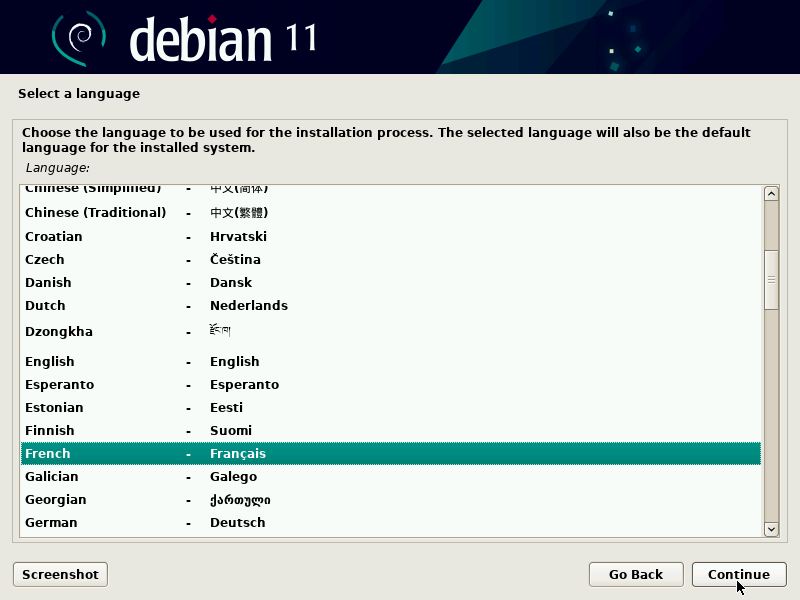
\includegraphics{res/02_langue.png}\strut
\end{minipage} & \begin{minipage}[t]{0.27\columnwidth}\raggedright
3. Locale : France\\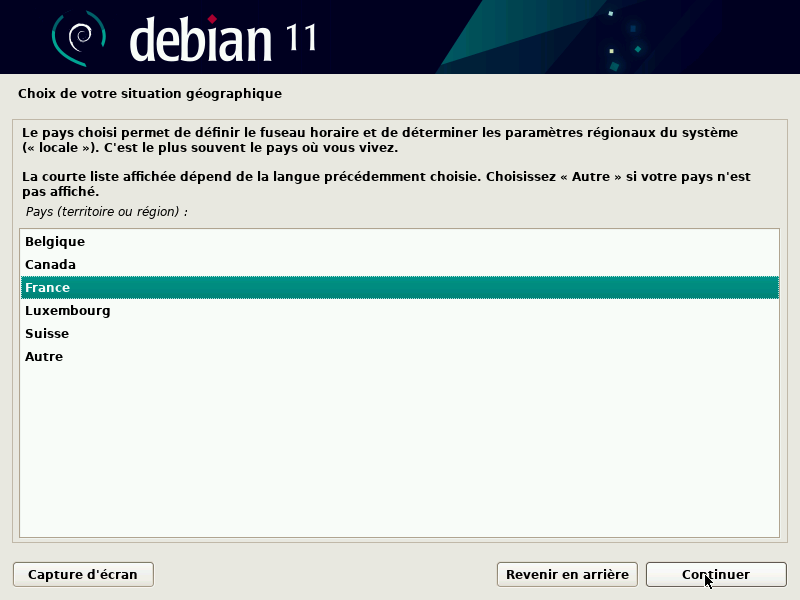
\includegraphics{res/03.png}\strut
\end{minipage}\tabularnewline
\begin{minipage}[t]{0.27\columnwidth}\raggedright
4. Clavier français\\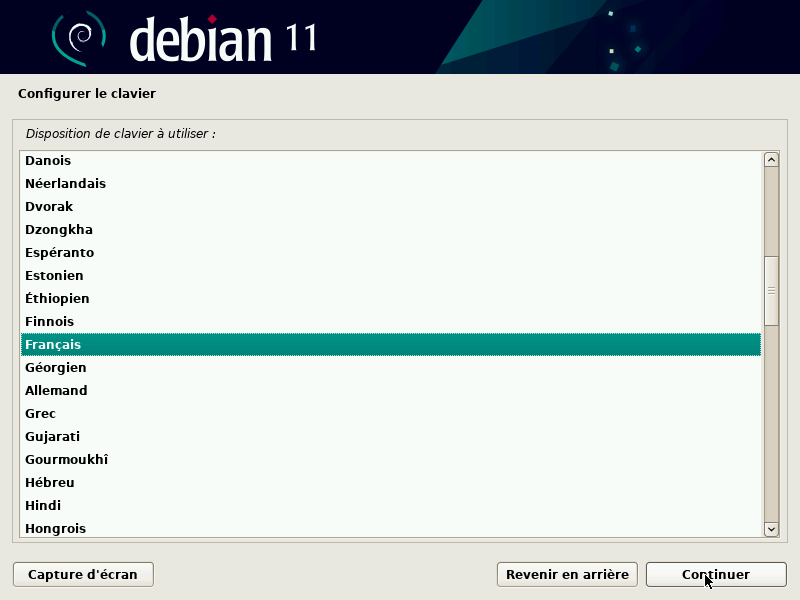
\includegraphics{res/04_clavier.png}\strut
\end{minipage} & \begin{minipage}[t]{0.37\columnwidth}\raggedright
5. Problème réseau :
configurer\\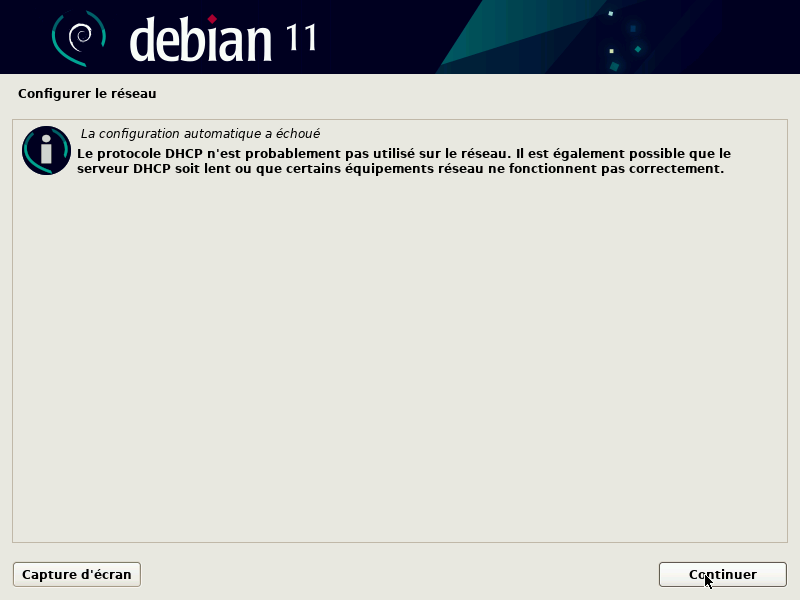
\includegraphics{res/05_pb_dhcp.png}\strut
\end{minipage} & \begin{minipage}[t]{0.27\columnwidth}\raggedright
6. Choisir de ne pas
configurer\\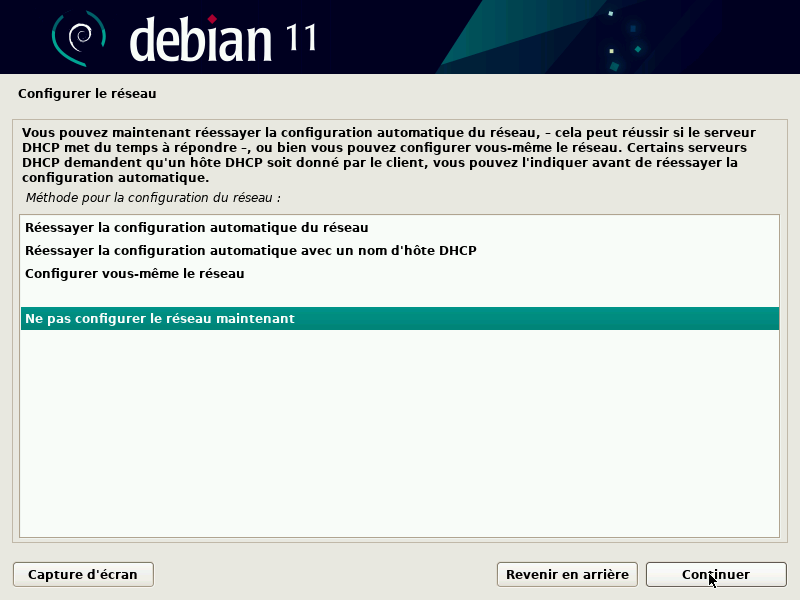
\includegraphics{res/06_ignorer_reseau.png}\strut
\end{minipage}\tabularnewline
\bottomrule
\end{longtable}

    \begin{longtable}[]{@{}lll@{}}
\toprule
\endhead
\begin{minipage}[t]{0.27\columnwidth}\raggedright
7. Nommer la machine \texttt{veil-debian-202-}\emph{\texttt{XX}} avec
\emph{\texttt{XX}} en fonction du numéro de votre
place\\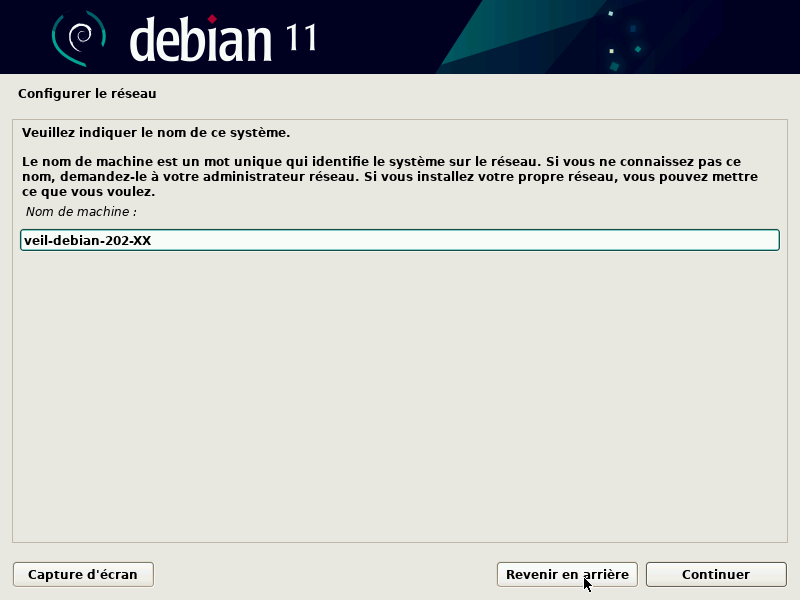
\includegraphics{res/07_nom_machine.png}\strut
\end{minipage} & \begin{minipage}[t]{0.37\columnwidth}\raggedright
8. Mot de passe \textbf{root} :
\texttt{12345678!}\\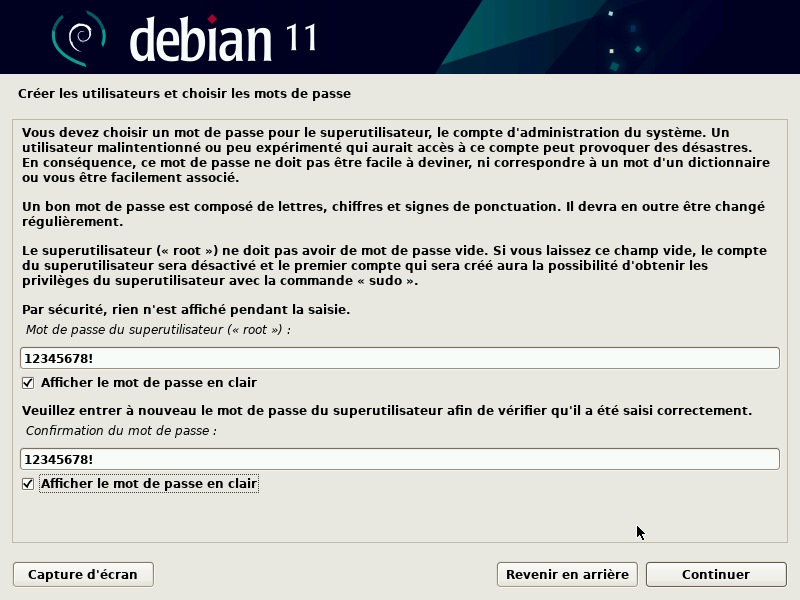
\includegraphics{res/08_mdp_root.png}\strut
\end{minipage} & \begin{minipage}[t]{0.27\columnwidth}\raggedright
9. Créer un premier utilisateur appelé \texttt{NSI} (et pas
\texttt{NSI\ XX} comme la capture
d'écran\ldots)\\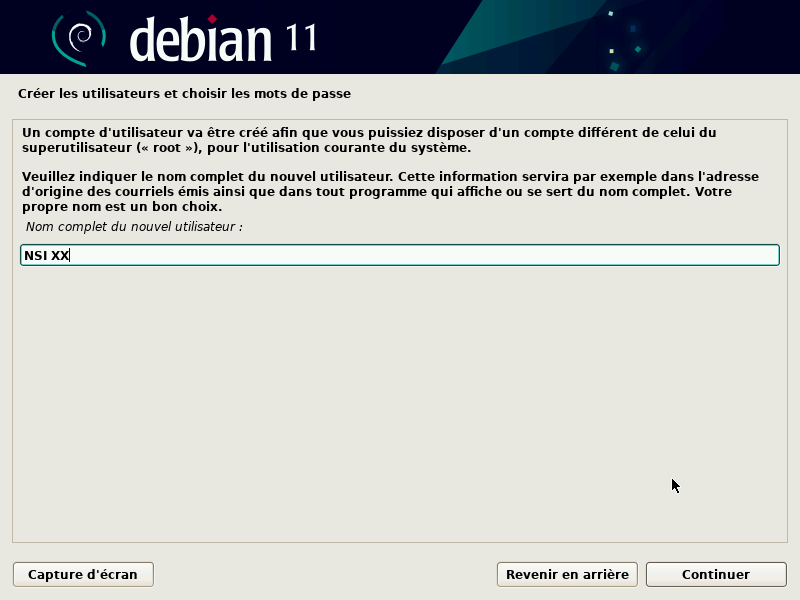
\includegraphics{res/09_id_user.png}\strut
\end{minipage}\tabularnewline
\begin{minipage}[t]{0.27\columnwidth}\raggedright
10. Valider l'identifiant
\texttt{nsi}\\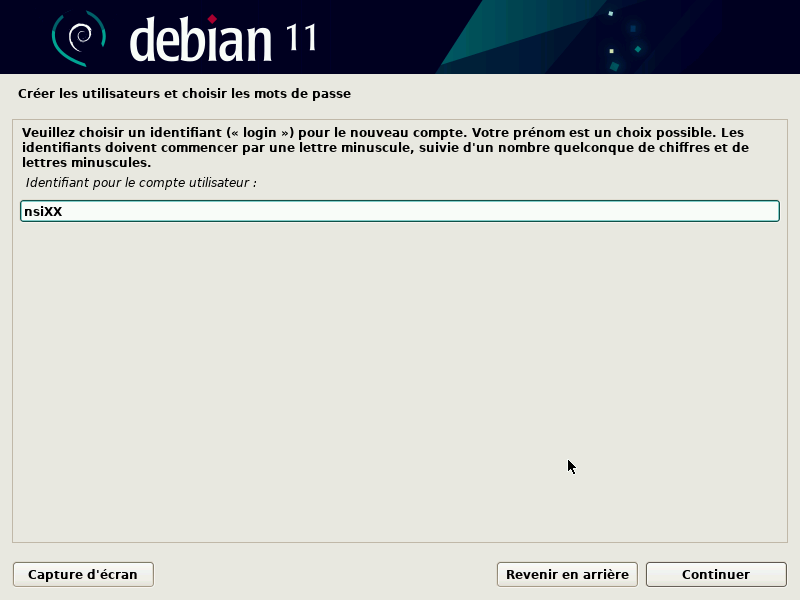
\includegraphics{res/10_id_user.png}\strut
\end{minipage} & \begin{minipage}[t]{0.37\columnwidth}\raggedright
11. Mot de passe de l'utilisateur \texttt{nsi} :
\texttt{nsi}\\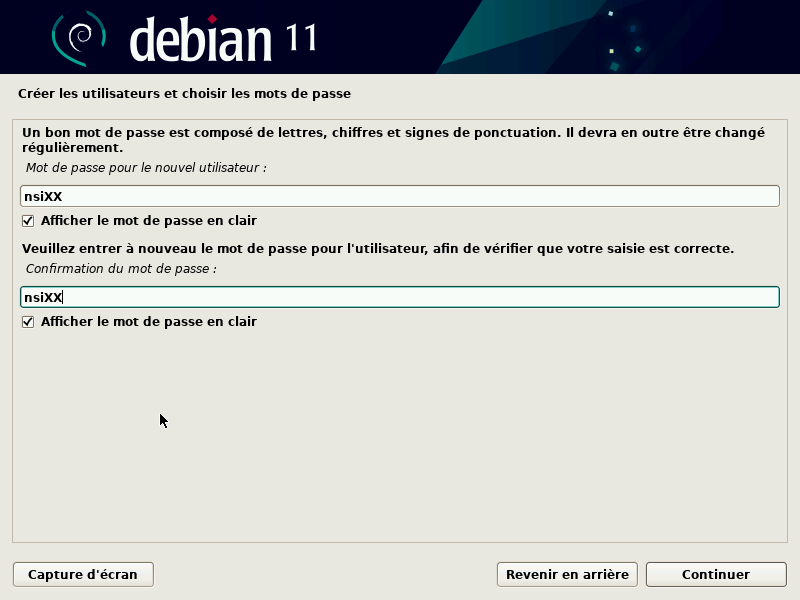
\includegraphics{res/11_mdp_user.png}\strut
\end{minipage} & \begin{minipage}[t]{0.27\columnwidth}\raggedright
12. Partitionner les disques de façon
manuelle\\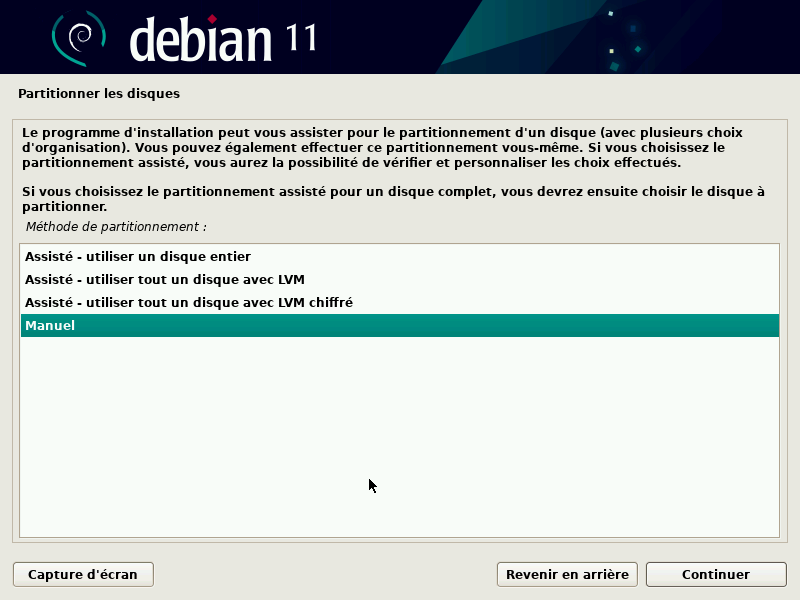
\includegraphics{res/12_partition_manuelle.png}\strut
\end{minipage}\tabularnewline
\bottomrule
\end{longtable}

    \hypertarget{partie-2---partitionner-le-disque}{%
\subsubsection{Partie 2 - Partitionner le
disque}\label{partie-2---partitionner-le-disque}}

    \begin{longtable}[]{@{}lll@{}}
\toprule
\endhead
\begin{minipage}[t]{0.27\columnwidth}\raggedright
1. Pour chaque partition de la liste\ldots{}
\\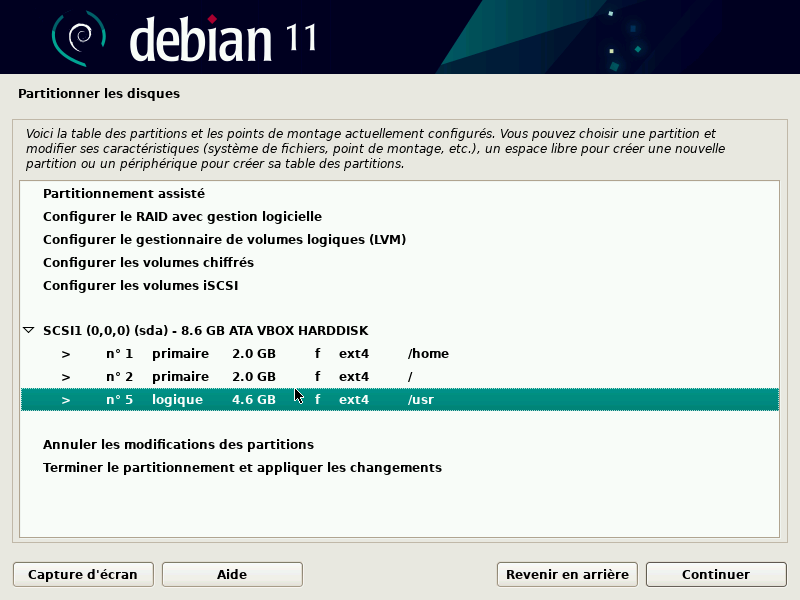
\includegraphics{res/13.png}\strut
\end{minipage} & \begin{minipage}[t]{0.37\columnwidth}\raggedright
2. \ldots la \textbf{supprimer} (et
oui!)\\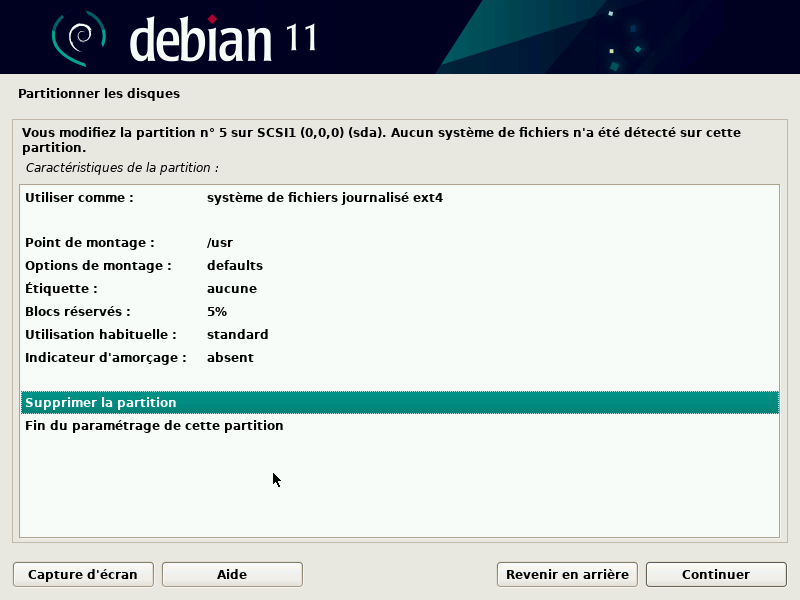
\includegraphics{res/14.png}\strut
\end{minipage} & \begin{minipage}[t]{0.27\columnwidth}\raggedright
3. Choisir l'unique espace vide ainsi créé
\\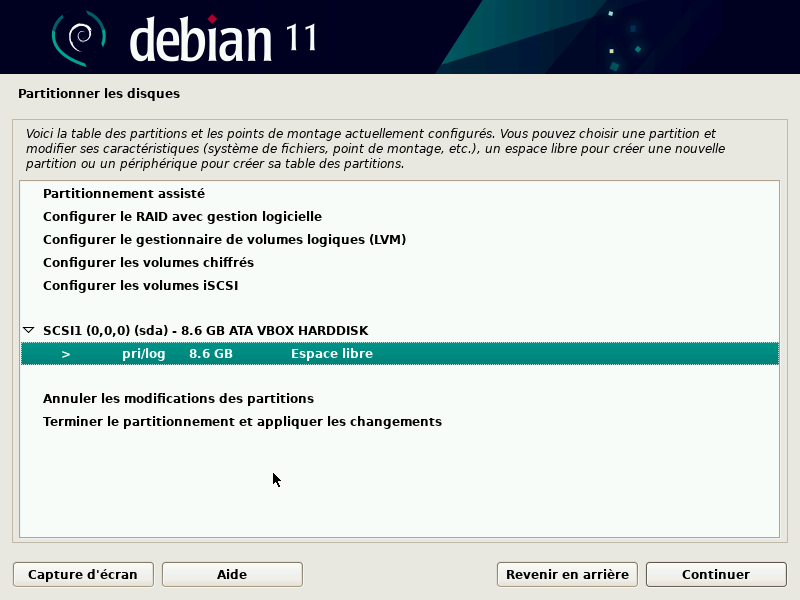
\includegraphics{res/15_zero_part.png}\strut
\end{minipage}\tabularnewline
\begin{minipage}[t]{0.27\columnwidth}\raggedright
4. Créer la \textbf{première} partition
\\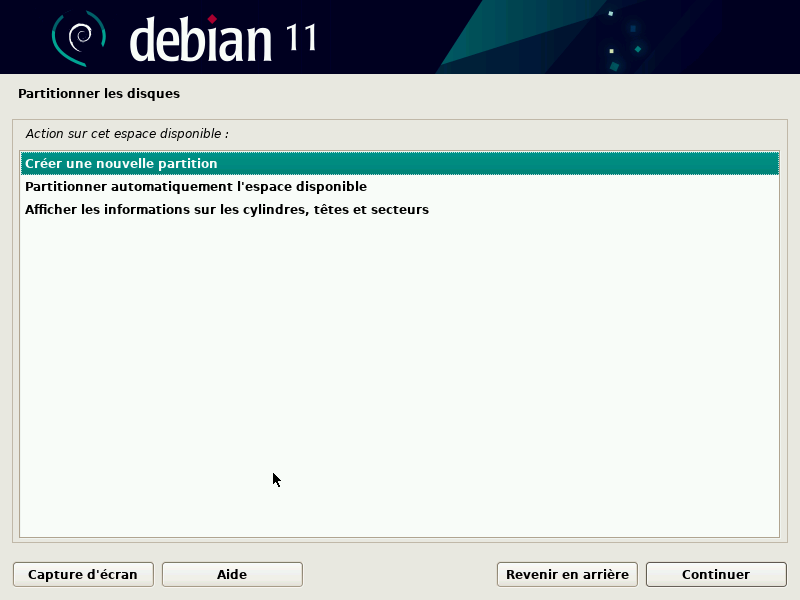
\includegraphics{res/16_creer.png}\strut
\end{minipage} & \begin{minipage}[t]{0.37\columnwidth}\raggedright
5. Saisir une petite taille de 100 Mo :
\texttt{100MB}\\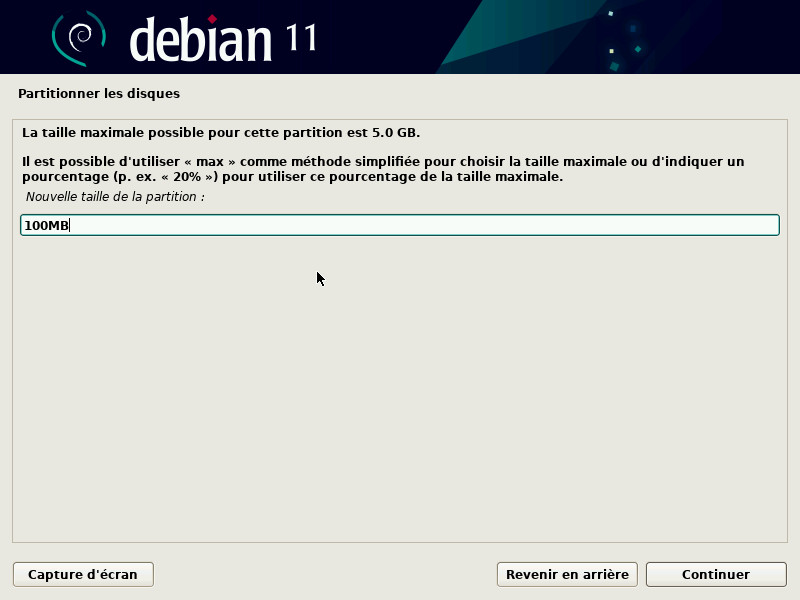
\includegraphics{res/50.png}\strut
\end{minipage} & \begin{minipage}[t]{0.27\columnwidth}\raggedright
6. Et une partition de type
\texttt{Primaire}\\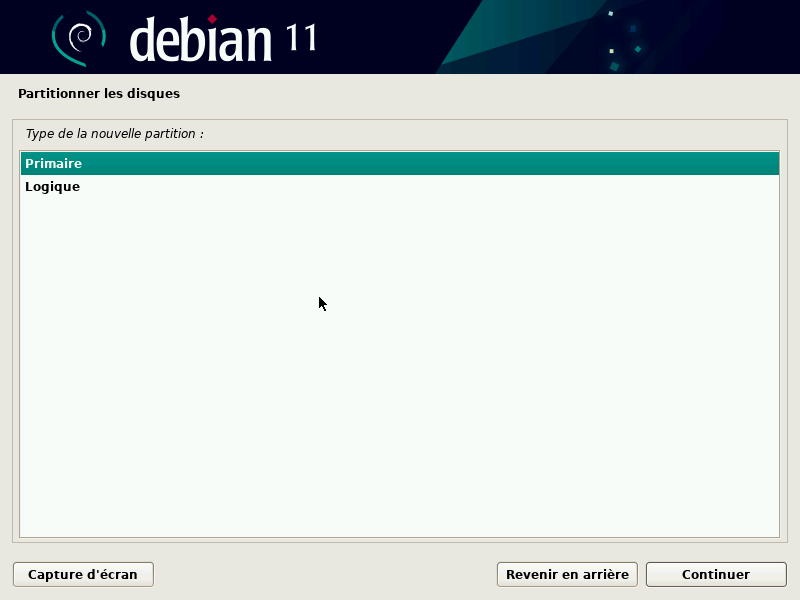
\includegraphics{res/51.png}\strut
\end{minipage}\tabularnewline
\bottomrule
\end{longtable}

    \begin{longtable}[]{@{}lll@{}}
\toprule
\endhead
\begin{minipage}[t]{0.27\columnwidth}\raggedright
7. Puis choisir Utiliser comme :
\ldots{}\\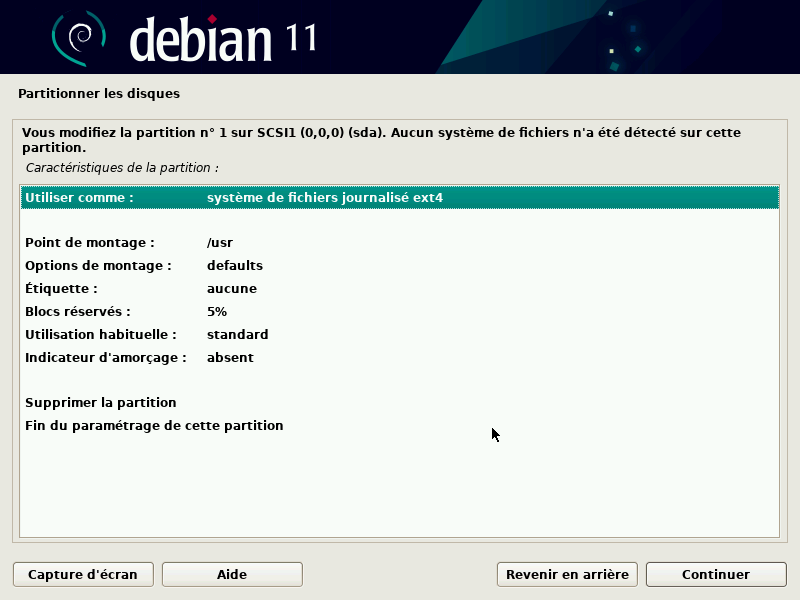
\includegraphics{res/53.png}\strut
\end{minipage} & \begin{minipage}[t]{0.37\columnwidth}\raggedright
8. \texttt{UEFI}(pas d'image\ldots)\strut
\end{minipage} & \begin{minipage}[t]{0.27\columnwidth}\raggedright
9. Puis dans le nouvel espace libre, créer la \textbf{deuxième}
partition\\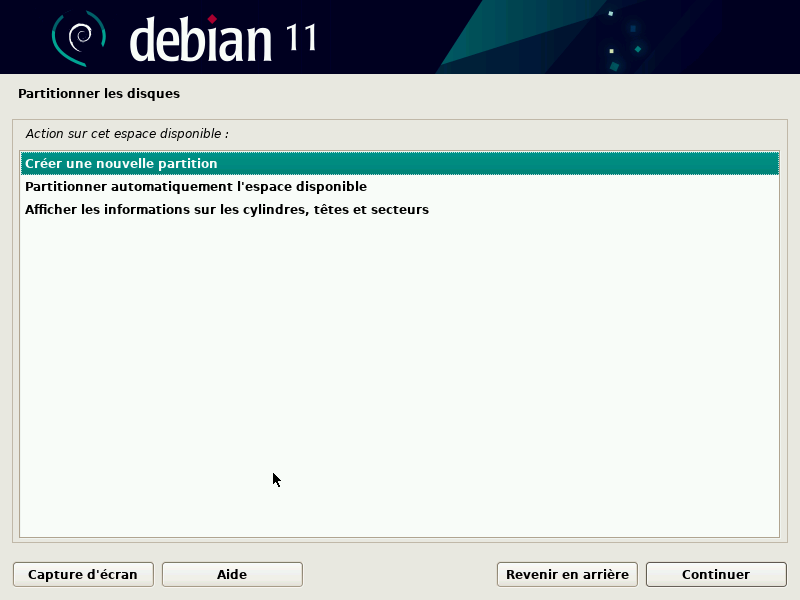
\includegraphics{res/16_creer.png}\strut
\end{minipage}\tabularnewline
\begin{minipage}[t]{0.27\columnwidth}\raggedright
10. de taille \texttt{50GB}\\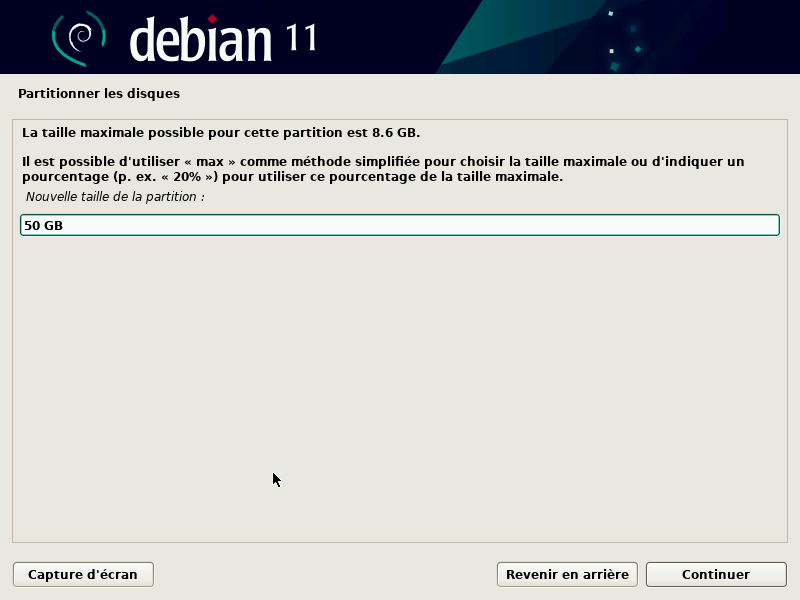
\includegraphics{res/17.png}\strut
\end{minipage} & \begin{minipage}[t]{0.37\columnwidth}\raggedright
11. De type Primaire\\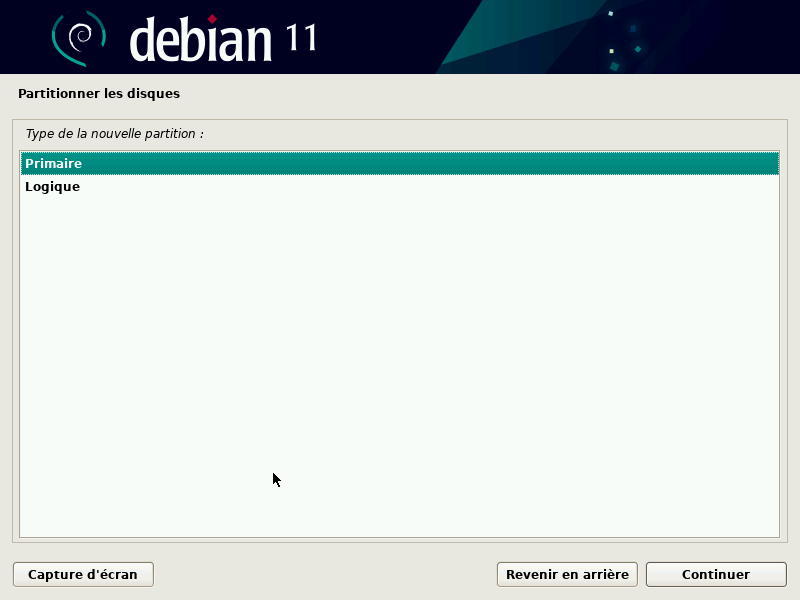
\includegraphics{res/18.png}\strut
\end{minipage} & \begin{minipage}[t]{0.27\columnwidth}\raggedright
12. Au début de l'espace vide\\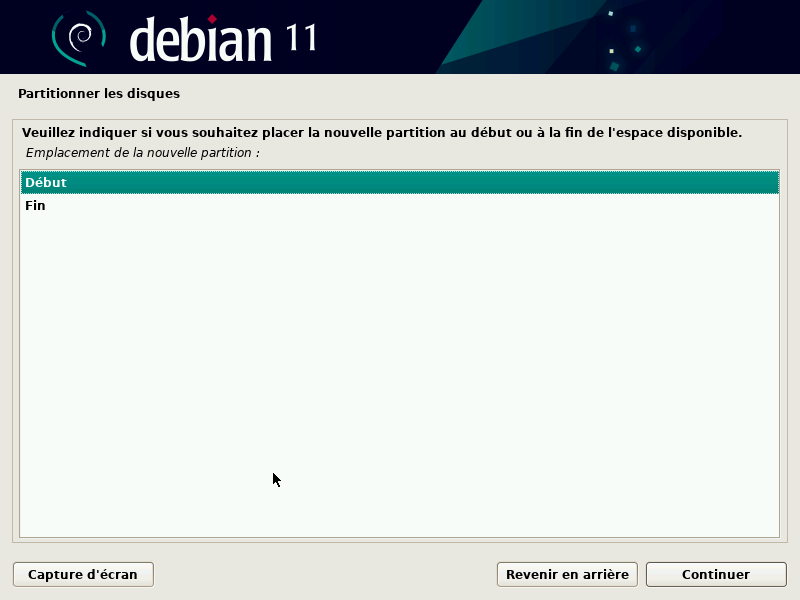
\includegraphics{res/19.png}\strut
\end{minipage}\tabularnewline
\bottomrule
\end{longtable}

    \begin{longtable}[]{@{}lll@{}}
\toprule
\endhead
\begin{minipage}[t]{0.27\columnwidth}\raggedright
13. Vérifier que le point de montage est bien
\texttt{/}\\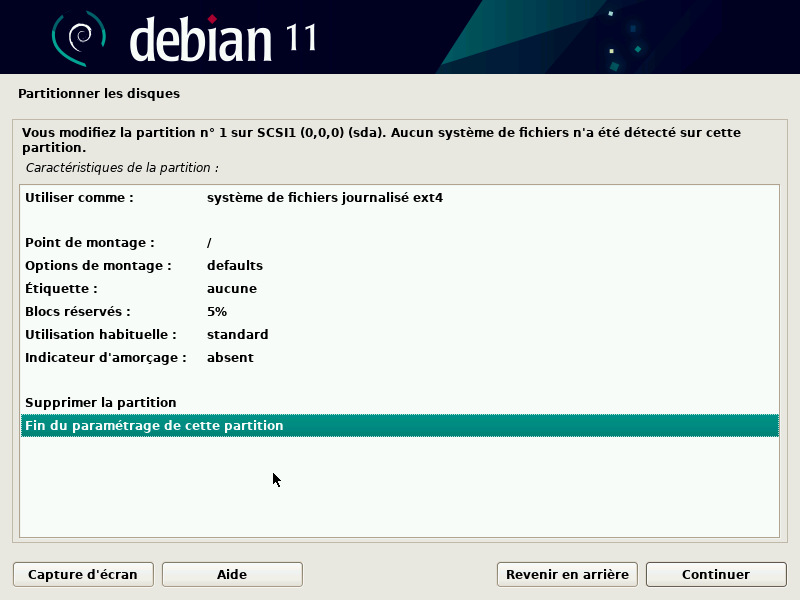
\includegraphics{res/20.png}\strut
\end{minipage} & \begin{minipage}[t]{0.37\columnwidth}\raggedright
14. Dans le nouvel espace vide, créer la \textbf{troisième} nouvelle
partition\ldots{} \\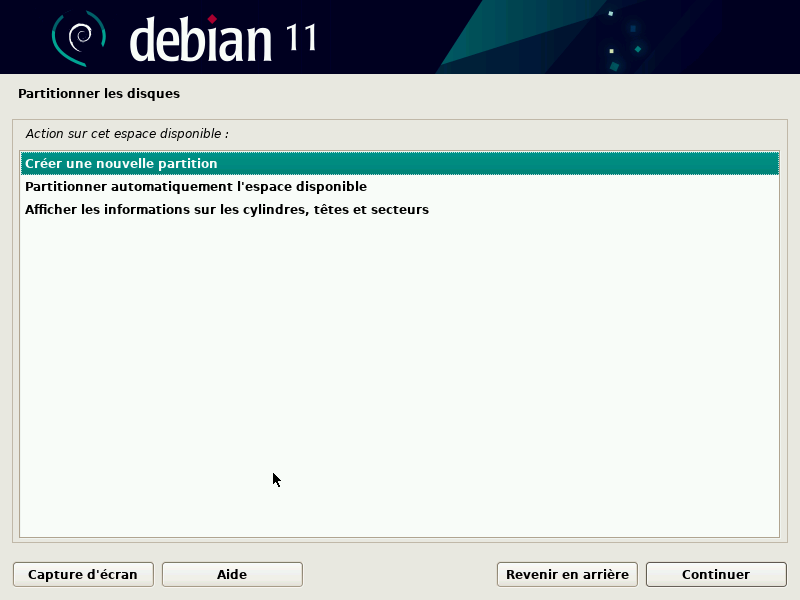
\includegraphics{res/21_swap.png}\strut
\end{minipage} & \begin{minipage}[t]{0.27\columnwidth}\raggedright
15. \ldots de taille
\texttt{4GB}\ldots{}\\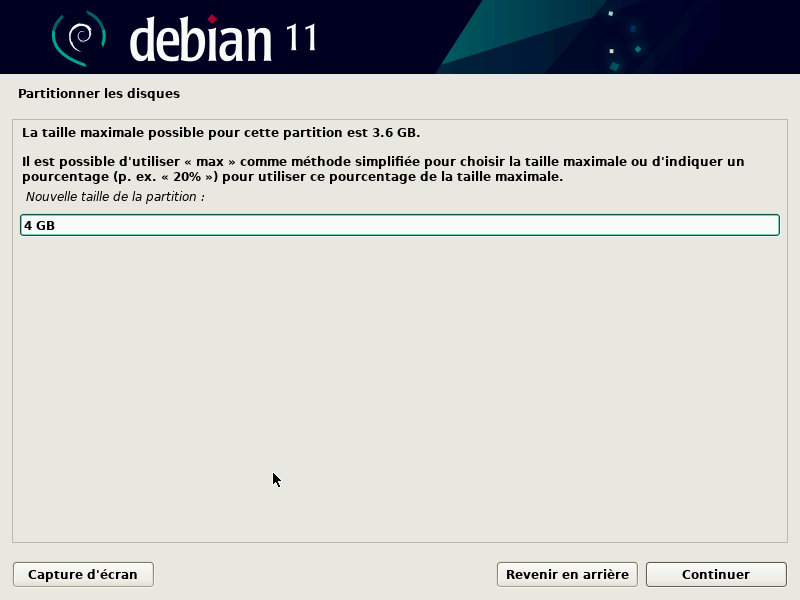
\includegraphics{res/22.png}\strut
\end{minipage}\tabularnewline
\begin{minipage}[t]{0.27\columnwidth}\raggedright
16. \ldots de type \texttt{Logique} (attention, la capture d'écran ne
correspond pas)\ldots{} \\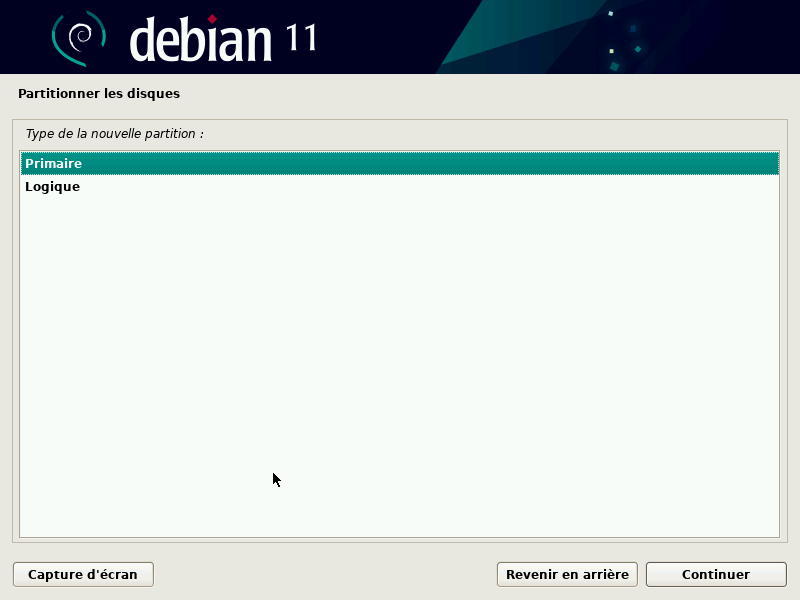
\includegraphics{res/23.png}\strut
\end{minipage} & \begin{minipage}[t]{0.37\columnwidth}\raggedright
17. \ldots au debut du disque\ldots{}\\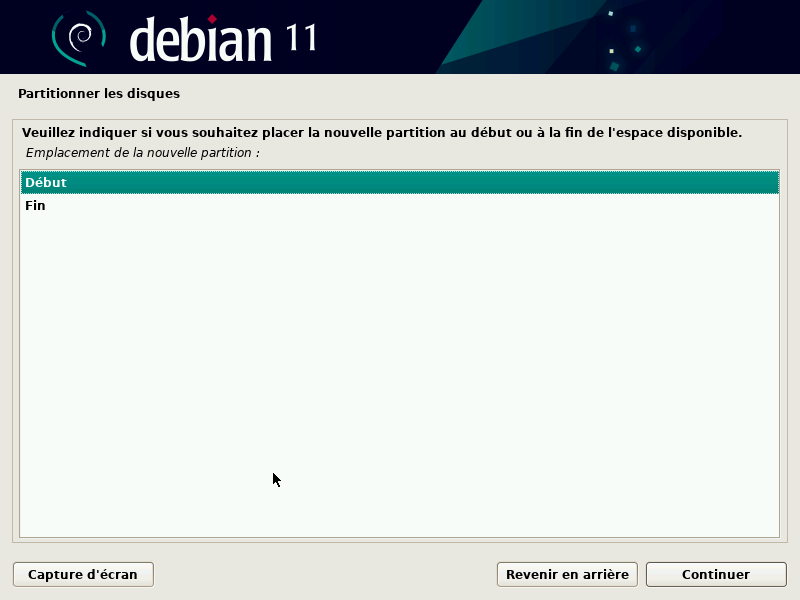
\includegraphics{res/19.png}\strut
\end{minipage} & \begin{minipage}[t]{0.27\columnwidth}\raggedright
18. Modifier
\texttt{utiliser\ comme}\ldots{}\\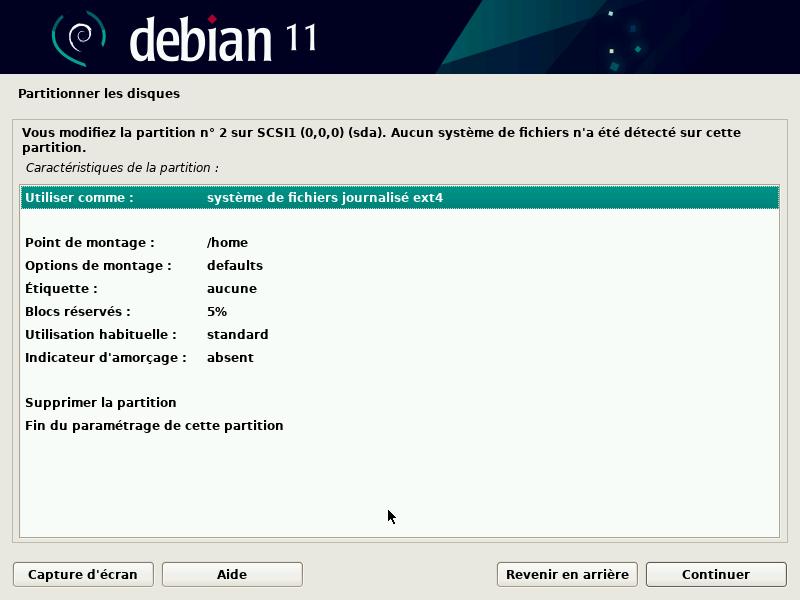
\includegraphics{res/24.png}\strut
\end{minipage}\tabularnewline
\bottomrule
\end{longtable}

    \begin{longtable}[]{@{}lll@{}}
\toprule
\endhead
\begin{minipage}[t]{0.27\columnwidth}\raggedright
19. \ldots et choisir
\texttt{espace\ d\textquotesingle{}échange\ ("swap")}\\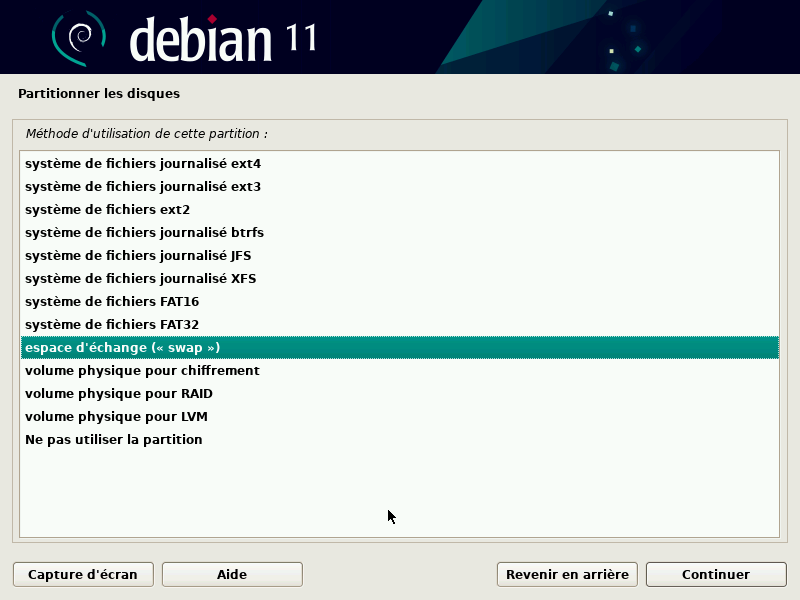
\includegraphics{res/25.png}\strut
\end{minipage} & \begin{minipage}[t]{0.37\columnwidth}\raggedright
20. Finir de paramétrer cette partition
\\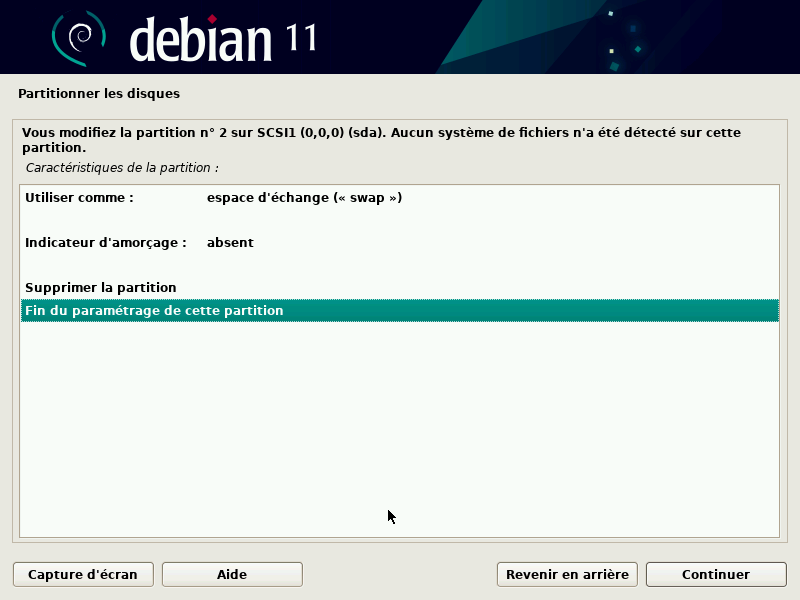
\includegraphics{res/26.png}\strut
\end{minipage} & \begin{minipage}[t]{0.27\columnwidth}\raggedright
21. Enfin, créer la \textbf{quatrième et dernière} partition dans
l'espace vide restant\\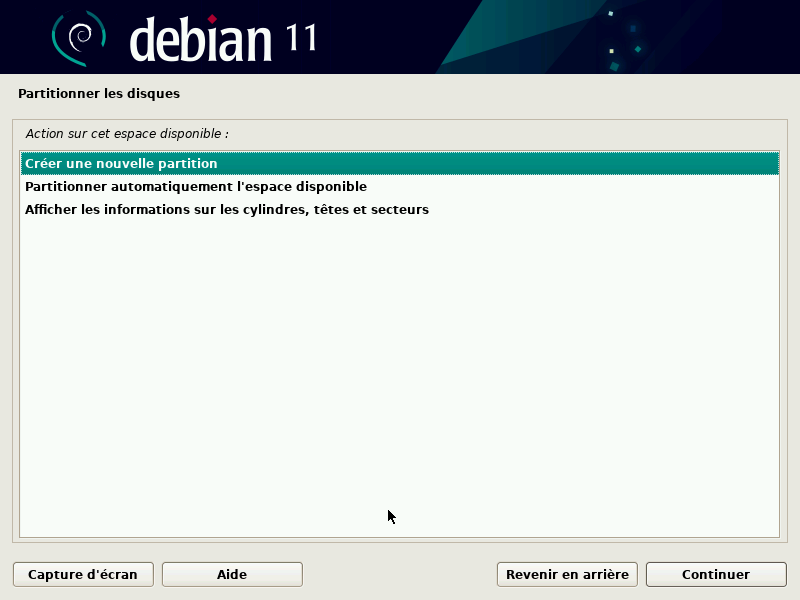
\includegraphics{res/27_home.png}\strut
\end{minipage}\tabularnewline
\begin{minipage}[t]{0.27\columnwidth}\raggedright
22. Laisser la plus grande taille
possible\\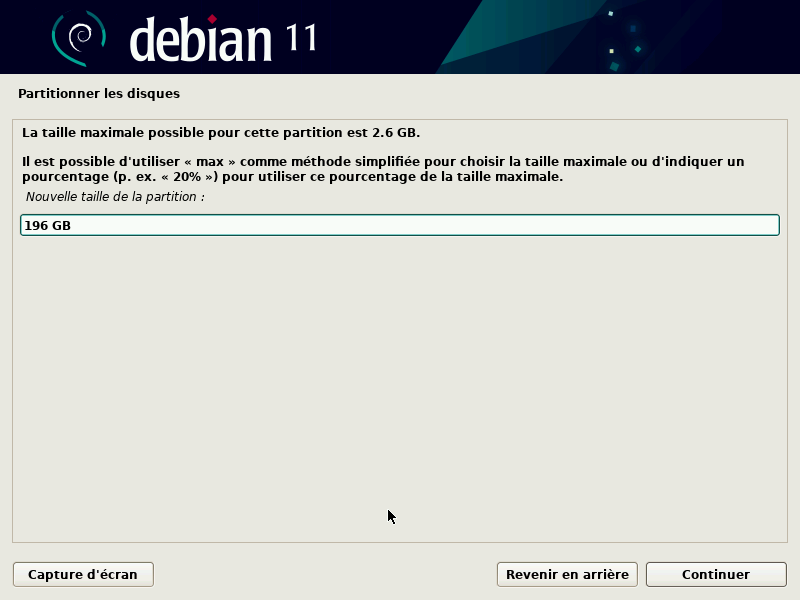
\includegraphics{res/28.png}\strut
\end{minipage} & \begin{minipage}[t]{0.37\columnwidth}\raggedright
23. Choisir de type
\texttt{Primaire}\ldots{}\\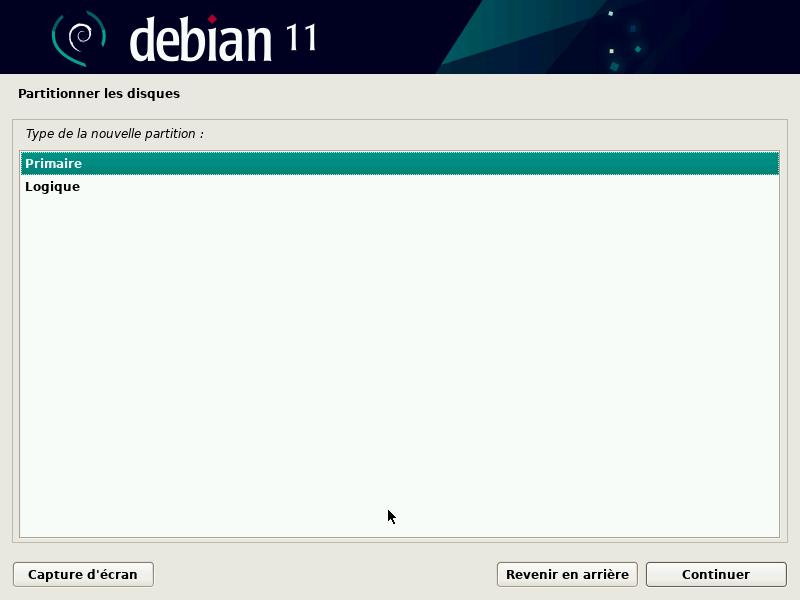
\includegraphics{res/29.png}\strut
\end{minipage} & \begin{minipage}[t]{0.27\columnwidth}\raggedright
24. Après avoir vérifié que le point de montage est bien \texttt{/home},
finir le paramétrage de cette partition
\\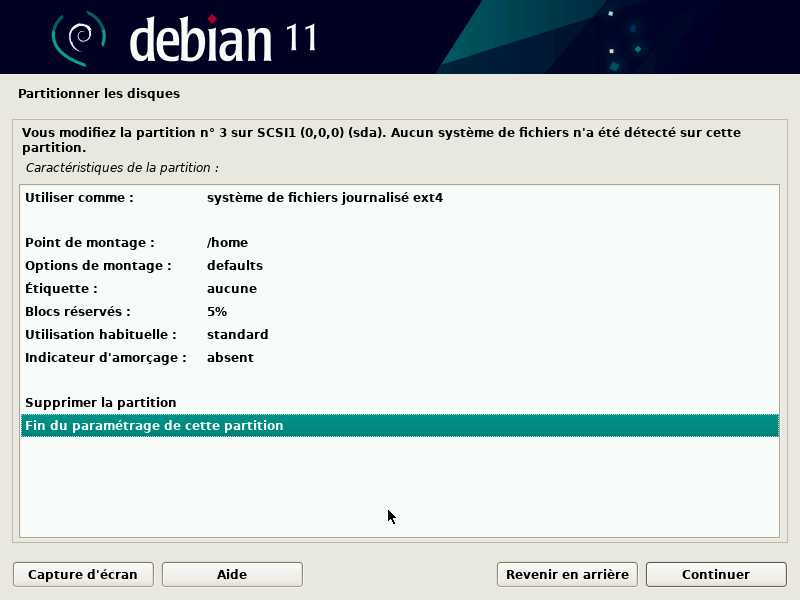
\includegraphics{res/30.png}\strut
\end{minipage}\tabularnewline
\bottomrule
\end{longtable}

    \hypertarget{attention}{%
\subsubsection{Attention !}\label{attention}}


\includegraphics{res/stop_hand.png}

\begin{enumerate}
\def\labelenumi{\arabic{enumi}.}
\setcounter{enumi}{24}
\tightlist
\item
  La configuration des partitions est terminée\ldots{} \textbf{mais}
  pour \emph{valider} cette étape longue, \textbf{appeler le
  professeur}.
\end{enumerate}

    \begin{longtable}[]{@{}lll@{}}
\toprule
\endhead
\begin{minipage}[t]{0.27\columnwidth}\raggedright
26. Terminer le partitionnement et valider les
changements\\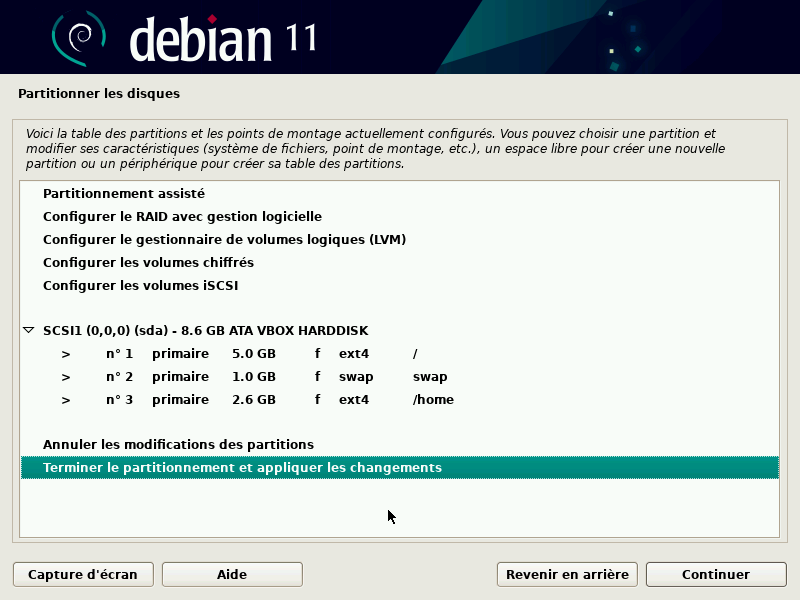
\includegraphics{res/31_terminer.png}\strut
\end{minipage} & \begin{minipage}[t]{0.37\columnwidth}\raggedright
27. Appliquer les changements en choisissant
\texttt{oui}\\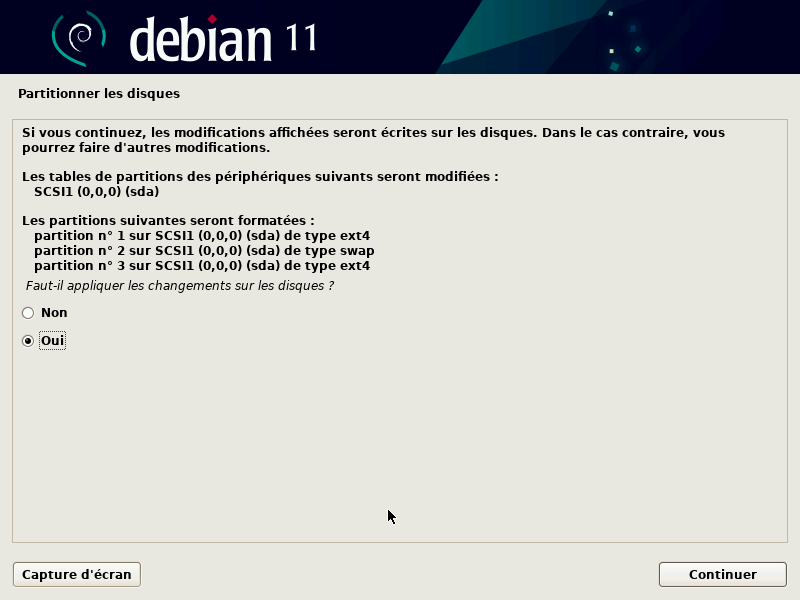
\includegraphics{res/32_ok.png}\strut
\end{minipage} & \begin{minipage}[t]{0.27\columnwidth}\raggedright
\strut
\end{minipage}\tabularnewline
\bottomrule
\end{longtable}

    \hypertarget{partie-3---finaliser-linstallation}{%
\subsubsection{Partie 3 - Finaliser
l'installation}\label{partie-3---finaliser-linstallation}}

    \begin{longtable}[]{@{}lll@{}}
\toprule
\endhead
\begin{minipage}[t]{0.27\columnwidth}\raggedright
1. Ne pas analyser d'autres supports :
\texttt{Non}\\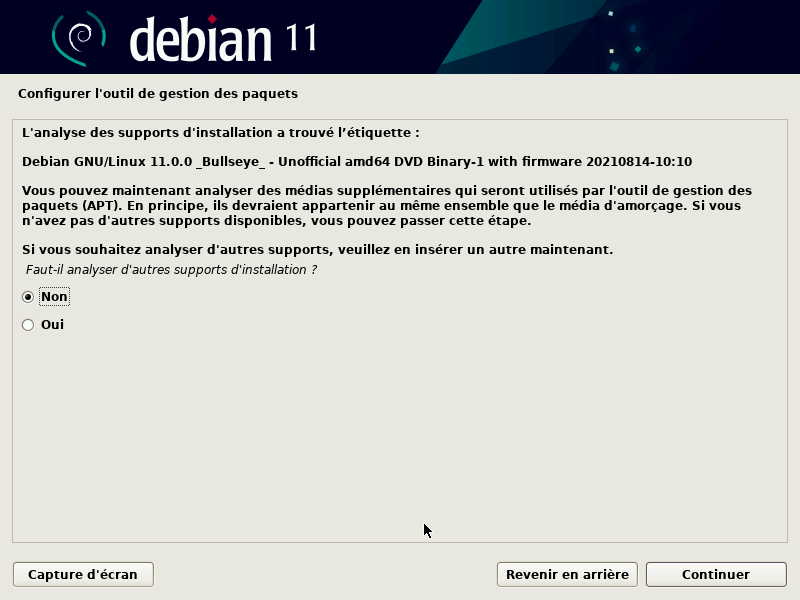
\includegraphics{res/33.png}\strut
\end{minipage} & \begin{minipage}[t]{0.37\columnwidth}\raggedright
2. Ne pas utiliser un miroir réseau :
\texttt{Non}\\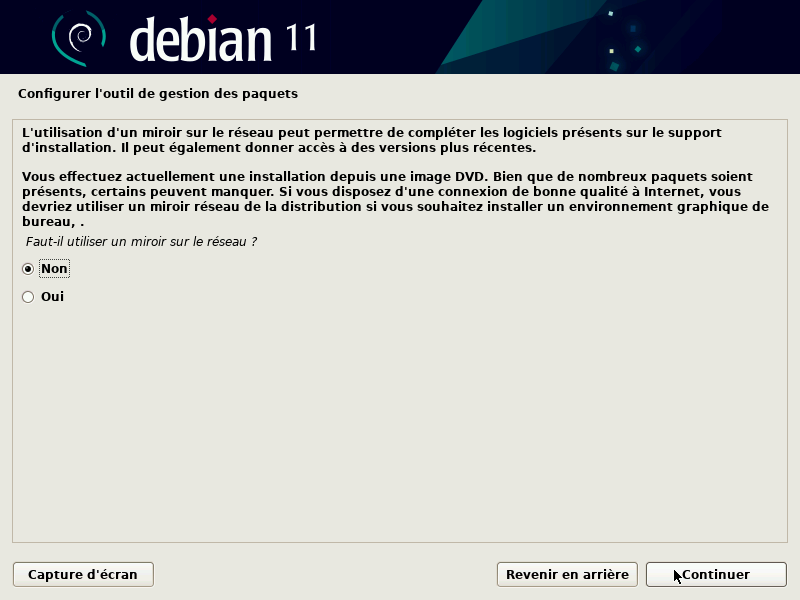
\includegraphics{res/34.png}\strut
\end{minipage} & \begin{minipage}[t]{0.27\columnwidth}\raggedright
3. Ne pas participer à l'étude statistique sur l'utilisation des
paquets\\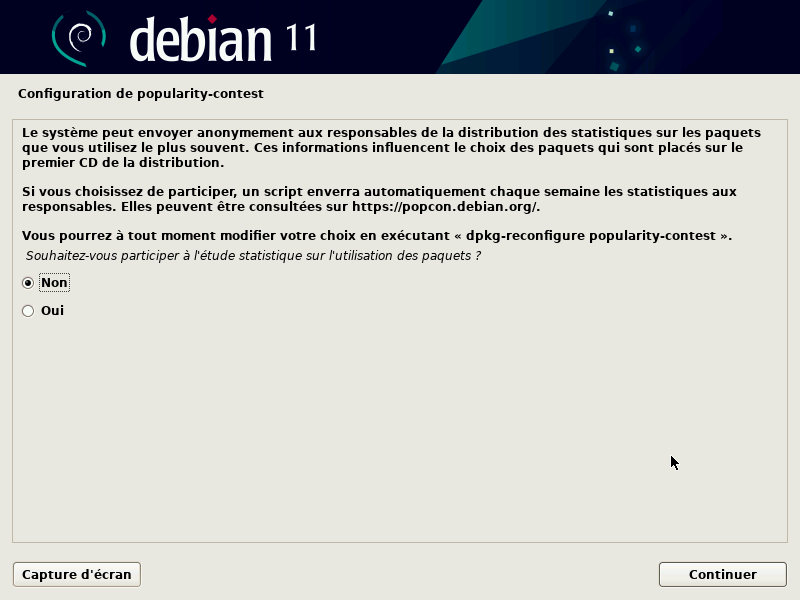
\includegraphics{res/35.png}\strut
\end{minipage}\tabularnewline
\begin{minipage}[t]{0.27\columnwidth}\raggedright
4. Choisir l'environnement de bureau Debian, Gnome et les utilitaires
usuels\\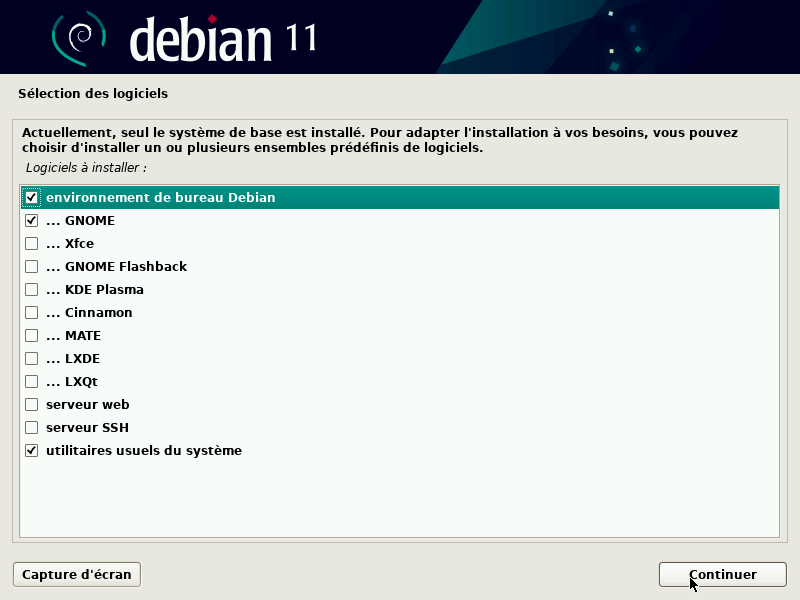
\includegraphics{res/36_choix.png}\strut
\end{minipage} & \begin{minipage}[t]{0.37\columnwidth}\raggedright
5. Installation du système d'exploitataion\ldots{} c'est très long ! (je
n'ai pas eu le temps de faire une capture (sic)\strut
\end{minipage} & \begin{minipage}[t]{0.27\columnwidth}\raggedright
6. Installer le programme de démarrage GRUB sur la partition UEFI
(première partition créée)\\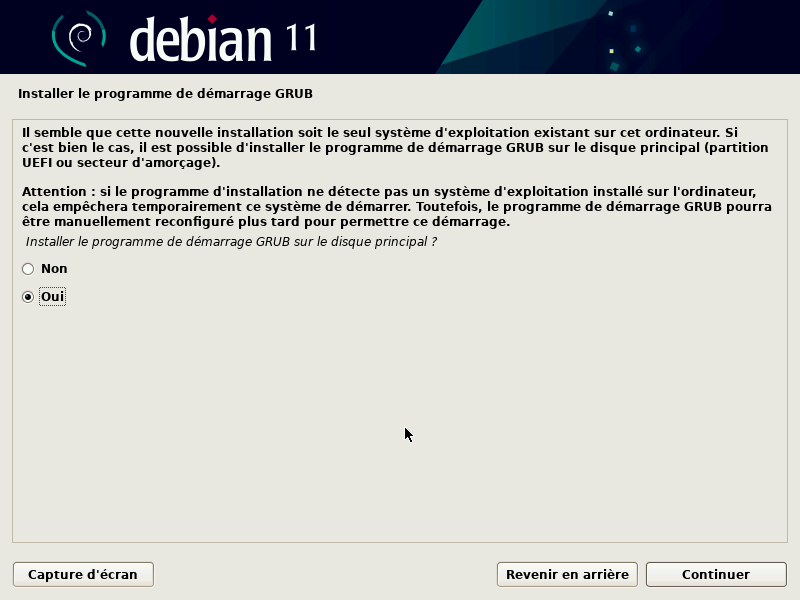
\includegraphics{res/37.png}\strut
\end{minipage}\tabularnewline
\bottomrule
\end{longtable}

    Et là, deux possibilités :

    \begin{longtable}[]{@{}ll@{}}
\toprule
Ça redémarre & Ça ne redémarre pas\ldots{}\tabularnewline
\midrule
\endhead
vide&%
\includegraphics{res/giphy_baby.gif} &
vide%\includegraphics{res/giphy_boom.webp}
\tabularnewline
\bottomrule
\end{longtable}

    \hypertarget{configurer-le-systuxe8me-dexploitation}{%
\subsection{Configurer le système
d'exploitation}\label{configurer-le-systuxe8me-dexploitation}}

    \hypertarget{tuxe9luxe9charger-les-fichiers-nuxe9cessaires}{%
\subsubsection{Télécharger les fichiers
nécessaires}\label{tuxe9luxe9charger-les-fichiers-nuxe9cessaires}}

    \begin{itemize}
\tightlist
\item
  \texttt{source.list}
\item
  \texttt{vscodium.list}
\item
  \texttt{product.json}
\item
  \texttt{.profile}
\item
  \texttt{filius.deb}
\item
  \texttt{logisim-evolution.deb}
\end{itemize}

    \hypertarget{changer-la-ruxe9solution-de-luxe9cran}{%
\subsubsection{Changer la résolution de
l'écran}\label{changer-la-ruxe9solution-de-luxe9cran}}

    \#TODO

    \hypertarget{configurer-les-duxe9pots}{%
\subsubsection{Configurer les dépots}\label{configurer-les-duxe9pots}}

    \hypertarget{mettre-uxe0-jour-le-source.list}{%
\paragraph{Mettre à jour le
source.list}\label{mettre-uxe0-jour-le-source.list}}

Dans un Terminal :

\begin{itemize}
\tightlist
\item
  passer en mode \emph{super utilisateur}
\item
  copier le fichier \texttt{source.list} dans le dossier
  \texttt{/etc/apt/}
\item
  créer le répertoire `/etc/source.list.d/
\item
  copier le fichier \texttt{vscodium.list} dans le dossier
  \texttt{/etc/apt/source.list.d/}
\end{itemize}

\begin{verbatim}
nsi@veil-debian00:~$ su
Mot de passe : 
root@veil-debian00:~# cp source.list /etc/apt/
root@veil-debian00:~# mkdir /etc/apt/source.lidt.d/
root@veil-debian00:~# cp vscodium.list /etc/apt/source.list.d/
\end{verbatim}

    \hypertarget{mettre-uxe0-jour-si-besoin}{%
\paragraph{Mettre à jour si besoin}\label{mettre-uxe0-jour-si-besoin}}

Toujours en \emph{super utilisateur}, mettre à jour la liste des paquets
et mettre à jour le système si besoin :

\begin{verbatim}
root@veil-debian00:~# apt update
root@veil-debian00:~# apt upgrade
\end{verbatim}

    \hypertarget{installer-les-paquets}{%
\paragraph{Installer les paquets}\label{installer-les-paquets}}

    Toujours en \emph{super utilisateur}, installer les paquets suivants:

\begin{itemize}
\tightlist
\item
  \texttt{mu-editor}
\item
  \texttt{vim}
\item
  \texttt{vlc}
\item
  \texttt{gimp}
\item
  \texttt{inkscape}
\item
  \texttt{codium}
\item
  \texttt{snapd}
\end{itemize}

grâce (par exemple) à la commande :

\begin{verbatim}
root@veil-debian00:~# apt install mu-editor
\end{verbatim}

\textbf{(astuce)} : utiliser %↑ et ⭾ (
  flêche du haut et tabulation%)

    \hypertarget{installer-par-.deb}{%
\subsubsection{Installer par .deb}\label{installer-par-.deb}}

    Installer les deux logiciels \texttt{.deb} téléchargés :

\begin{itemize}
\tightlist
\item
  \texttt{logisim-evolution}
\item
  \texttt{filius}
\end{itemize}

En \emph{super utilisateur} :

\begin{verbatim}
root@veil-debian00:~# dpkg -i filius.deb
root@veil-debian00:~# dpkg -i logisim-evolution.deb
root@veil-debian00:~# apt -f install
\end{verbatim}

    \hypertarget{installer-par-snap}{%
\subsubsection{Installer par snap}\label{installer-par-snap}}

    Installer deux derniers logiciels grâces aux dépots \texttt{snap} :

\begin{verbatim}
nsi@veil-debian00:~$ snap install freeplane-mindmapping
nsi@veil-debian00:~$ snap install drawio
\end{verbatim}


    % Add a bibliography block to the postdoc
    
    
    
\end{document}
